\documentclass[a4paper,11pt]{article}
\usepackage[utf8]{inputenc}
\usepackage[english]{babel}

\usepackage{amsfonts}
\usepackage{amsmath}
\usepackage{amsthm}
\usepackage{caption}
\usepackage{epsfig}
\usepackage[top=3cm, bottom=3cm, left=4cm, right=4cm]{geometry}
\usepackage{graphicx}
\usepackage{pgfplots}
\usepackage{pst-grad}
\usepackage{pst-plot}
\usepackage{subcaption}

\bibliographystyle{acm}

\pgfplotsset{compat=newest}

%opening
\title{A task-based approach to stencil computations}
\author{Nicolet, Victor}

\begin{document}
\pagenumbering{gobble}
\begin{minipage}{3.5cm}
  
\includegraphics[width=3.5cm]{logox.jpg}
  \begin{center}
  Ecole polytechnique\\
  Promotion X2012\\
  NICOLET Victor
  \end{center}
\end{minipage}

\vspace{3cm}

\begin{center}

{\Large \textbf{RAPPORT DE STAGE DE RECHERCHE}}\\
\vspace{1cm}
{\Large\textbf{A task-based approach to stencil computations}}\\
\makebox{\rule{12cm}{0.4pt}}\\
\vspace{1cm}
{\large NON CONFIDENTIEL}\\

\end{center}
\vspace{4cm}
\begin{tabular}{p{.55\textwidth}r}
 D\'epartement d'informatique & \\
 Champ: & INF591 \\
 Directeur de stage :´& BOURNEZ Olivier \\
 Maitre de stage :& COHEN Albert \\
 Dates du stage: & 23 mars 2015-17 juillet 2015 \\
 Nom et adresse de l'organisme : & D\'epartement d'informatique \\
 & Ecole Normale Sup\'erieure \\
 & 45 rue d'Ulm \\
 & 75005 Paris \\
 & France
\end{tabular}

\clearpage
\newpage
\null\vspace{5cm}
\section*{Acknowledgements}
I would like to express my gratitude to my internship advisor, professor Albert Cohen,
for giving me the opportunity to work in the team, his advice and discussions. I also
want to thank Nhat Minh-L\^e for his help and availability with Libkpn and general advice,
and also all those who worked on the project, Adrien Guatto and Robin Morisset. \\
Finally, I would like to thank the whole PARKAS team for their welcome during my stay.

\clearpage
\newpage
\null
\vspace{5cm}
\begin{abstract}
The main purpose of this internship is to study and implement new applications in a complete 
runtime system for Kahn process networks, Libkpn, developed in the Inria/ENS PARKAS team. \\
The implementation of 1-d jacobi stencil application in the special case of small iteration numbers,
using a special tiling technique, shows better performance than implementations using the 
state-of-the-art OpenMP4 model for shared-memory concurrent programs. 
\end{abstract}
\newpage
\pagenumbering{arabic}
\tableofcontents
\newpage

\section{Introduction}
\subsection{Motivation}
Multi-core processors with shared memory are now common in devices ranging from mobile
phones to supercomputers. There has been a growing interest in providing frameworks
to help the common programmer to build efficient programs that would execute
on multi-core architectures. Though there have been different approaches, they all try to
address the problem of :
\begin{itemize}
 \item  providing the tools to program parts that can be solved concurrently.
 \item  implementing an overall control and coordination mechanism.
\end{itemize}
Here, we will address computational problems in which breaking the program into parts for
concurrent execution is nontrivial. During the computation, time is often spent in nested
loops, with iterations depending on each other. When splitting or “tiling” the iteration space to 
distribute the work among the different cores, some problems arise :
\begin{itemize}
 \item the program must stay correct. Breaking a program into parts and modifying its control flow
 and data flow must be done cautiously. Not all transformations are legal : while some parts of the
 program can be done in parallel, others must be executed sequentially.
 \item the architecture has its limitations. We must keep in mind that inter-processor 
 communication is very costly and must be avoided, and that memory usage is a determinant 
 factor in a program's performance.
\end{itemize}
Previous research has provided many solutions to this problem, aiming to improve 
parallelism and reduce synchronization and communication overheads. Compilers and domain
specific languages can provide automatic parallelization today,thanks to abstractions like 
the polyhedral model \cite{bondhugula_automatic_2008}, or simpler models with assumptions 
over the inputs \cite{ragan-kelley_halide:_2013}. \\
However these solutions are not always optimal.
We will provide a simple tiling for time iterated stencil applications that yields good
performance on unidimensional jacobi (1-d jacobi), a simple time-iterated stencil. \\
The scheduling of the different parts of the program is also an interesting field of research.
We will compare the performance static scheduling of for loops used in OpenMP to the
dynamic scheduling of a task network in Libkpn, the library developed in PARKAS team.
The results show that it is possible to equal the performance of hand-tuned OpenMP implementations
with the task-based approach using Libkpn.


\subsection{Contribution and outline}
The PARKAS team, in which I did my internship, is focused on synchronous Kahn parallel networks. There 
is two main research topics : the definition of high-level languages for embedded systems that provide
synchronous data-flow concurrency, and efficient compilation for synchronous and concurrent designs 
targeting modern shared-memory parallel processors. \\
I worked more specifically on Libkpn : a library that provides the user lightweight tasks and
first-class dependencies to implement any network of tasks for parallel execution, based
on the model of Kahn process networks \cite{kahn_semantics_1974}.\\
The main purpose of my internship was to show that tasks and dynamic scheduling can
perform as well as static scheduling,  widely used in shared-memory models such
as OpenMP. Libkpn has already proved its efficiency on classic linear algebra kernels such
as Cholesky decomposition and streaming applications. But other real world applications
in image processing and scientific computation use computationally intensive kernels, and these
applications need high-performance parallelization.\\
I initially focused on learning about the state of the art in parallel programming and concurrency
models on shared-memory architectures. This included research on program transformations and dynamic
scheduling. \\
In the first application I had to develop, my goal was to use inner parallelism in an image processing
pipeline, Harris Corner Detection, but this did not lead to convincing results. Then my focus moved 
on to a stencil application, 1-d jacobi. We hoped that using tasks and dynamic scheduling, we would 
improve performance by taking advantage of reuse between successive tiles. My work was an exploration
of the potential applications for Libkpn, thus a part of the project and a continuation of previous 
articles.\\
\vspace{1cm}
The following report presents first the general background necessary to understand the tools and and models
I used during my internship. We discuss the results of the experiments with the different Harris Corner
Detection implementations. Finally, the main results with 1-d jacobi are presented, with the tiling 
strategy and task model used.


%********************************************************
%  BACKGROUND
%********************************************************
\section{Background}
\subsection{Stencil applications}
Stencil applications are a broad family of compute intensive applications, widely used in
the graphic or scientific domain. We can characterize them by an update of a point in a
grid, using neighboring points. They have properties that make them a good subject for
optimization. We will take as example the jacobi stencil in one spatial dimension as example 
(see figure~\ref{jbi1d_code:naive}).
\paragraph{Characterization}
A stencil computation is a time-iterated nearest-neighbor computation that operates on
each point in a grid and updates each grid point using data in its neighboring points, in
recent time steps. We use the stencil characterization presented in \cite{bandishti_tiling_2012} :
\begin{itemize}
 \item  Grid points are updated using the values of neighboring points in previous and recent
time-steps. Nested loops have always a time-step iteration as outermost loop, and
we assume there is no horizontal dependence between statements (the values of a
points does not depend directly on the value of other points in the same time-step).
\item If we have $d$ spatial dimensions, the computations uses a $d + 1$ dimensional grid, the
outermost dimension being the time dimension. In the implementation, the grid will
be reduced to the spatial grid only, for memory efficiency.
\item  The stencil can always be written in a single-statement of the following form, with
a stencil function $f$ :
\[value_p[t + 1] = f (value_p[t], value_{neighbors\_of\_p}[t])\]
\end{itemize}
A stencil computation computes the stencil for each point of the grid over many time
steps. Theses applications are quite simple to implement using nested loops, but they are
subject to many problems of optimization. These are mainly loop transformations, since
the computation is contained in the nested loops. \\
We will consider the following stencil function $f$ in a one-dimensional grid $\mathbb{G}$, with a data
grid $A_\mathbb{G}$:
\[\mathbb{G} = [0, N - 1] \subset N \ , \ 
A_\mathbb{G} \subset \mathbb{R} \ , \ 
f (A) = (A[t, i] + [A[t, i - 1] + A[t, i + 1])/3
\]
The stencil computation can be written simply with two nested loops and one statement,
using a time-space grid (figure~\ref{jbi1d_code:naive}) or two data grids 
(figure~\ref{jbi1d_code:mem}). The use of a bi-dimensional array in the first example
with a time dimension allows to nest the two loops perfectly and permit simple transformations. 
A \textbf{perfect loop nest} is a set of nested loops in which all statements appear in the innermost
loop.
But this is very memory-inefficient, and the time dimension in the array is superfluous. \\
The second form of the program adds a second statement to swap data in arrays. However, there 
is more statements and the second loop depends on the first one, creating additional dependencies.

\begin{figure}
 \begin{subfigure}{.5\textwidth}
  \begin{verbatim}
   for (t = 0; t < T; t++)
      for (i = 1; i < N-1; i++)
          S1: A[t+1][i] = 0.333 *
                  (A[t][i-1] +
                     A[t][i] +
                    A[t][i+1]);
  \end{verbatim}
  \caption{Perfectly nested 1-d jacobi}
  \label{jbi1d_code:naive} 
 \end{subfigure}
 \begin{subfigure}{.5\textwidth}
  \begin{verbatim}
  for (t = 0; t < T; t++)
      for (i = 1; i < N-1; i++)
          S1 : B[i] = 0.3333 * 
                 (A[i-1] + 
                  A[i] + 
                  A[i+1]);
      for (i = 0; i < N; i++)
          S2 : A[i] = B[i];   
  \end{verbatim}
  \caption{Imperfectly nested 1-d jacobi}
  \label{jbi1d_code:mem}
 \end{subfigure}
 \caption{1-d Jacobi}
 \label{jbi1d_code}
\end{figure}

In the remaining of the report, we will consider mainly stencil computations, or at least 
computations that are structured alike : an outer “time” loop and dependencies from 
one time step to another, spanning along the iteration space and with some dependencies having
non-negative components along the spatial dimension. The graphs will present a 
time or iterations dimension, representing the domain of the outer loop, and a space dimension
for the inner loop.


\subsection{Program transformations and polyhedral framework}
Most highly computational algorithms are built with a set of nested loop and some statements, 
accessing and reading data. The program transformations we need to perform
concern mostly these loops. In figure~\ref{jbi1d_code}, we have one outer-loop iterating on 
time, and an inner loop on the spatial dimension.
\paragraph{Data dependency} In the perfectly nested loop in figure~\ref{jbi1d_code:naive} the
dynamic instances of statement $S1$ at $(i, t)$ reads data that has been written by $S1$ at 
$(t − 1, i)$, $(t − 1, i − 1)$ and $(t − 1, i + 1)$. We call this a \textit{data dependency} :
a dynamic instance of a program statement refers to data of a preceding statement. We will refer 
simply to a \textit{dependency} since we are not interested in other kinds of dependencies.

\subsubsection{Loop transformations}
To exploit parallelism in the application, we have to modify the nested loops structure, while
ensuring the program still produces the correct output. We present some correct loop
transformations \cite{bacon_compiler_1994} to modify the program and produce the correct strategy.
\begin{itemize}
 \item  loop skewing can be useful to enable parallelism. Since it only changes loop bounds
	and alters accordingly the use of index variables, it is always legal to perform skewing
	on loops. Figure~\ref{jbi1d_tr:skewed} shows a skewed version of 1-d jacobi.
 \item  loop tiling is useful to improve cache performance. When performing loop tiling on
	an outer loop (containing other loops), we divide the iteration space into chunks and
	iterate over these parts. Figure~\ref{jbi1d_tr:tiled} show a tiling using tiles of
	size $64 \times 64$.
 \item 	loop distribution (or loop splitting, loop fission) can be used to distribute a single 
	loop into different loops. This can create perfect nested loops, or reduce the
	dependences in the nested loops. The inverse transformation is loop fusion.
\end{itemize}
Loop tiling and distribution legality is constrained by the dependences. We will speak of
tile dependencies when we perform tiling, and see that loop transformations alter theses
dependencies.
\begin{figure}
 \begin{subfigure}{.5\textwidth}
  \begin{verbatim}
for (t = 0; t < T; t++)
  for(i = t + 1; i < t+N-1; i++)
     S1 : B[i - t] = 0.3333 *
                 (A[i-1 - t] +
                  A[i - t] +
                  A[i+1 - t]);
  \end{verbatim}
  \caption{Skewed 1-d jacobi}
  \label{jbi1d_tr:skewed} 
 \end{subfigure}
 \begin{subfigure}{.5\textwidth}
  \begin{verbatim}
for(Tt = 0; tT < T; Tt+=64)
  for(Ti = 0; Ti < N; Ti+=64)
    for (t = Tt; t < Tt + 64; t++)
      for(i = Ti; i < Ti + 64; i++)
         S1 : B[i] = 0.3333 * (A[i-1] +
                     A[i] + A[i+1]);
  \end{verbatim}
  \caption{Tiled 1-d jacobi}
  \label{jbi1d_tr:tiled}
 \end{subfigure}
  \caption{1-d jacobi after loop transformations}
\end{figure}
Yet these transformations can be expressed in a more high level model, which will also
allows to find suitable transformations for parallelization. Programming manually transformed 
loops is a very tedious work and error prone. During my internship, I programmed
various tilings using manual loop transformations, but the goal today in high performance computing 
is to build automatic systems using the model described in the following paragraph.
Though I did not use it myself except for some experiments with Pluto \cite{bondhugula_automatic_2008}, 
I could not dissociate the optimization of iteration spaces
and tilings from this field of research, also very important in the team where I was working.

\subsubsection{Polyhedral model}
Simple transformations are easy to achieve without excessively complexifying the original
program. But when loop nests become more complicated, a mathematical framework can
prove useful to express loop skewing, tiling, distributing etc. We will express the properties
of our stencil applications in a linear-algebraic representation of programs, the polyhedral
model, and provide a brief description of it. Given a representation of a program, it will
be easier to express further transformations and show their validity.
This model has been proved very useful in automatic parallelization at compile time
\cite{bastoul_code_2004},
because it provides many abstractions to reason about program transformations.

\paragraph{Polyhedral representation of programs} A program is a set of dynamic instances
of statements. Each instance $S$ is defined by its iteration vector $\vec{i}$ containing the values
of the indexes of the loops containing the statement. When inner loop bounds depend
on outer indexes values, the set of iterations vectors representing different instances of a
statement define a polytope $D_s$ (see figure~\ref{poly:itspace}), the domain of the statement, with 
$m_s$ its dimensionality. In this model, we consider only convex iteration spaces.
\paragraph{Polyhedral dependencies} The difficulty of parallelizing stencil applications arises
when considering the dependencies between dynamic instances of the statements. Dependences are affine and
exact, and only carried by the time loops in our stencil applications.
The data dependence graph is a directed multi-graph, with each node $S_i$ representing a
statement and each edge $e \in E$ representing a dependence between statements $S_i$ and $S_j$ .
$e$ can be represented here a constant distance vector by analyzing the source and target
iterators in the domain $D_s$ .
In 1-d jacobi we have only 3 dependencies $\vec{d_1} = (−1, 1)$, $\vec{d_2} = (0, 1)$ and $\vec{d_3} = 
(1, 1)$
(figure~\ref{poly:deps}
\begin{figure}
 \begin{subfigure}{.5\textwidth}
  \[ D_{S1} : \begin{bmatrix}
               1&0\\-1&0\\0&1\\0&-1
              \end{bmatrix}
              \begin{pmatrix}
               i\\t
              \end{pmatrix}
              \geq
              \begin{pmatrix}
               1\\-(N-1)\\0\\-T
              \end{pmatrix}
   \]
   \caption{1-d jacobi original polytope}
   \label{poly:itspace}
 \end{subfigure}
 \begin{subfigure}{.5\textwidth}
  \begin{center}
  \psscalebox{1.0 1.0} % Change this value to rescale the drawing.
    {
    \begin{pspicture}(0,-0.74383867)(3.42,0.74383867)
    \psline[linecolor=black, linewidth=0.04, arrowsize=0.05291666666666667cm 2.0,arrowlength=1.4,arrowinset=0.0]{->}(1.6,-0.7296965)(0.8,0.0703035)
    \psline[linecolor=black, linewidth=0.04, arrowsize=0.05291666666666667cm 2.0,arrowlength=1.4,arrowinset=0.0]{->}(1.6,-0.7296965)(1.6,0.0703035)
    \psline[linecolor=black, linewidth=0.04, arrowsize=0.05291666666666667cm 2.0,arrowlength=1.4,arrowinset=0.0]{->}(1.6,-0.7296965)(2.4,0.0703035)
    \rput[bl](0.0,0.0703035){$\vec{d_1}$}
    \rput[bl](1.6,0.4703035){$\vec{d_2}$}
    \rput[bl](2.8,0.0703035){$\vec{d_3}$}
    \end{pspicture}
    }
    \end{center}
    \caption{1-d jacobi dependence vectors}
    \label{poly:deps}
 \end{subfigure}
\end{figure}

\subsubsection{Tiling}
  Tiling in stencil applications is a key transformation to improve locality,memory reuse
  and parallelism. There has been a considerable amount of research in this domain, and
  we present here a summary of previous work, as well as the goals we try to achieve.
  
  \newtheorem{depsdef}{Definition}
  \newtheorem{legality}{Tiling legality}
  
  \paragraph{Tiling legality} In figure~\ref{jbi1d_code:mem} we have an example of imperfectly-nested loops.
  It raises  more problems when searching for valid tiling hyperplanes. Using the polyhedral framework, 
  we have conditions provided in prior research, expressed in \cite{bondhugula_automatic_2008}. A 
  \textbf{legal tiling} is a tiling that ensures that we can construct a total order between tiles 
  for execution (there is no tiles that depend on each other) and provided inter-tile dependencies
  are satisfied, a tile can execute atomically.
  \begin{depsdef}
    A hyperplane for a statement $S_i$ is of the following form:
      \[\phi_{S_i}(\vec{x}) =  \vec{h} \cdot \vec{x} + h0 \]
  where $ \vec{x} \in D_s$ is an instance of the statement $S_i$, 
  $h0$ is the translation and $\vec{h}$ is the hyperplane normal vector.
  \end{depsdef}
  
  \begin{legality}
    Let $\phi_{S_i}$ be a one-dimensional affine transform for statement
    $S_i$. For ${\phi_{S_0} , .., \phi_{S_k}}$ to be a legal tiling hyperplane, 
    the following should hold for each edge $e$ from $S_i$ to $S_j$ :
    \[\phi_{S_j}(t) - \phi_{S_i}(s) \geq 0 \ , \ P_e\]
  \end{legality}
  In our example with only one statement, a legal tiling hyperplane with normal vector
  $⃗\vec{h} = (h_i, h_t$) must satisfy the following conditions :
  \[\vec{h} \cdot \vec{d_1} = h_t - h_i \geq 0 \ , \ 
  \vec{h} \cdot \vec{d_2} = h_t \geq 0 \ , \ 
  \vec{h} \cdot \vec{d_3} = h_i + h_t \geq 0\]
  Here rectangular tilings ($h_t = 0$ and $h_i > 0$) are not considered legal, unless 
  a space transformation is performed before.
  Parallel computations should minimize interprocessor communications and rectangular tilings are not 
  satisfactory when dependence vectors have negative components along the space dimension.

  \paragraph{Tiling for locality} The spatial dimensions of most problems involving stencil computations 
  are usually quite large, often larger than the cache sizes or other on-chip memory
  size. Parallelism is present along the spatial dimension, but tiling is necessary to improve
  data locality during the computation and the different memory speeds.\\
  The objective here is to fit the tile spatial domain into on-chip memory, potentially at
  different levels. The tiling concerns here the inner loops.

  \paragraph{Tiling for reuse} The goal is to work around the problem of limited memory bandwidth
  by using present memory as mush as possible before releasing it to memory levels with
  longer access delays. Many computations are throttled by this issue, an efficient schedule
  along the time dimension can dramatically improve the performances. Tiling only the inner
  loops to provide locality is not sufficient. But transforming the nested loops including the
  outer one can enhance memory reuse between different tiles.
  
  \paragraph{Tiling for communication-free parallelism} In current multiprocessor architectures,
  communication between processing units is costly and has to be avoided. Tiling for parallelism 
  implies finding calculations that can be executed at the same time and without
  data from other concurrent calculations. \\
  A tiling enables a tile-wise concurrent start if all that tiles along one dimension of the iteration
  space can be started concurrently. If tiles carry dependences along one dimension,
  they can not be started concurrently along this dimension. \\
  When dependences span the entire iteration space, there is often a trade-off between locality,
  memory reuse and and communication-free parallelism.

\subsubsection{Tiling techniques in previous research work}
  \paragraph{Skewed tiling} Skewing the iteration space is a standard tiling technique for time-
  iterated stencils along with rectangular space tiling. Visually speaking, figure~\ref{skewed-tiling}
  presents the shape of the tiles, parallelograms along the time dimension, and regular and legal
  tiling long the spatial dimensions. This improves memory reuse but creates inter-tiles
  dependencies along the space dimension, restricting parallelism to tile wavefronts along
  diagonals, and forbidding a concurrent start.

  \vspace{1cm}
  \begin{figure}[h]
    \begin{center}
    \psscalebox{.8 .8} % Change this value to rescale the drawing.
{
\begin{pspicture}(0,-4.12)(13.61,4.12)
\definecolor{colour0}{rgb}{0.003921569,0.003921569,0.003921569}
\definecolor{colour1}{rgb}{0.99607843,0.99607843,0.99607843}
\definecolor{colour2}{rgb}{0.49019608,0.49019608,0.49019608}
\definecolor{colour3}{rgb}{0.6862745,0.6862745,0.6862745}
\definecolor{colour4}{rgb}{0.84313726,0.84313726,0.84313726}
\definecolor{colour5}{rgb}{0.93333334,0.93333334,0.93333334}
\psframe[linecolor=colour0, linewidth=0.06, fillstyle=solid,fillcolor=colour1, dimen=outer](7.2,-3.32)(1.2,-4.12)
\pspolygon[linecolor=red, linewidth=0.04, fillstyle=solid,fillcolor=colour2](1.6,-2.52)(4.4,-2.52)(1.6,0.28)
\pspolygon[linecolor=red, linewidth=0.04, fillstyle=solid,fillcolor=colour3](4.4,-2.52)(6.8,-2.52)(3.6,0.68)(1.6,0.68)(1.6,0.28)
\pspolygon[linecolor=red, linewidth=0.04, fillstyle=solid,fillcolor=colour4](6.8,-2.52)(9.2,-2.52)(6.0,0.68)(3.6,0.68)
\pspolygon[linecolor=red, linewidth=0.04, fillstyle=solid,fillcolor=colour4](3.6,0.68)(1.6,0.68)(1.6,2.68)
\pspolygon[linecolor=red, linewidth=0.04, fillstyle=solid,fillcolor=colour5](11.6,-2.52)(8.4,0.68)(6.0,0.68)(9.2,-2.52)
\pspolygon[linecolor=red, linewidth=0.04, fillstyle=solid,fillcolor=colour5](6.0,0.68)(3.6,3.08)(1.6,3.08)(1.6,2.68)(3.6,0.68)
\pspolygon[linecolor=red, linewidth=0.04, fillstyle=solid,fillcolor=colour1](11.6,-2.52)(12.8,-2.52)(12.8,-1.32)(10.8,0.68)(8.4,0.68)
\pspolygon[linecolor=red, linewidth=0.04, fillstyle=solid,fillcolor=colour1](8.4,0.68)(6.0,3.08)(3.6,3.08)(6.0,0.68)
\pspolygon[linecolor=red, linewidth=0.04, fillstyle=solid,fillcolor=colour1](3.6,3.08)(1.6,3.08)(1.6,3.88)(2.8,3.88)
\psdots[linecolor=black, dotsize=0.2](2.0,1.08)
\psdots[linecolor=black, dotsize=0.2](2.0,1.88)
\psdots[linecolor=black, dotsize=0.2](2.8,1.88)
\psdots[linecolor=black, dotsize=0.2](2.8,1.08)
\psdots[linecolor=black, dotsize=0.2](2.8,2.68)
\psdots[linecolor=black, dotsize=0.2](2.0,2.68)
\psdots[linecolor=black, dotsize=0.2](2.0,0.28)
\psdots[linecolor=black, dotsize=0.2](2.8,0.28)
\psdots[linecolor=black, dotsize=0.2](2.0,-0.52)
\psdots[linecolor=black, dotsize=0.2](2.8,-0.52)
\psdots[linecolor=black, dotsize=0.2](2.0,-1.32)
\psdots[linecolor=black, dotsize=0.2](2.8,-1.32)
\psdots[linecolor=black, dotsize=0.2](3.6,-1.32)
\psdots[linecolor=black, dotsize=0.2](3.6,-0.52)
\psdots[linecolor=black, dotsize=0.2](3.6,0.28)
\psdots[linecolor=black, dotsize=0.2](3.6,1.08)
\psdots[linecolor=black, dotsize=0.2](3.6,1.88)
\psdots[linecolor=black, dotsize=0.2](3.6,2.68)
\psdots[linecolor=black, dotsize=0.2](4.4,2.68)
\psdots[linecolor=black, dotsize=0.2](4.4,1.88)
\psdots[linecolor=black, dotsize=0.2](4.4,1.08)
\psdots[linecolor=black, dotsize=0.2](4.4,0.28)
\psdots[linecolor=black, dotsize=0.2](4.4,-0.52)
\psdots[linecolor=black, dotsize=0.2](4.4,-1.32)
\psdots[linecolor=black, dotsize=0.2](5.2,-1.32)
\psdots[linecolor=black, dotsize=0.2](5.2,-0.52)
\psdots[linecolor=black, dotsize=0.2](5.2,0.28)
\psdots[linecolor=black, dotsize=0.2](5.2,1.08)
\psdots[linecolor=black, dotsize=0.2](5.2,1.88)
\psdots[linecolor=black, dotsize=0.2](5.2,2.68)
\psdots[linecolor=black, dotsize=0.2](6.0,2.68)
\psdots[linecolor=black, dotsize=0.2](6.0,1.88)
\psdots[linecolor=black, dotsize=0.2](6.0,1.08)
\psdots[linecolor=black, dotsize=0.2](6.0,0.28)
\psdots[linecolor=black, dotsize=0.2](6.0,-0.52)
\psdots[linecolor=black, dotsize=0.2](6.0,-1.32)
\psdots[linecolor=black, dotsize=0.2](6.8,-1.32)
\psdots[linecolor=black, dotsize=0.2](6.8,-0.52)
\psdots[linecolor=black, dotsize=0.2](6.8,0.28)
\psdots[linecolor=black, dotsize=0.2](6.8,1.08)
\psdots[linecolor=black, dotsize=0.2](6.8,1.88)
\psdots[linecolor=black, dotsize=0.2](6.8,2.68)
\psdots[linecolor=black, dotsize=0.2](7.6,2.68)
\psdots[linecolor=black, dotsize=0.2](7.6,1.88)
\psdots[linecolor=black, dotsize=0.2](7.6,1.08)
\psdots[linecolor=black, dotsize=0.2](7.6,0.28)
\psdots[linecolor=black, dotsize=0.2](7.6,-0.52)
\psdots[linecolor=black, dotsize=0.2](7.6,-1.32)
\psdots[linecolor=black, dotsize=0.2](8.4,-1.32)
\psdots[linecolor=black, dotsize=0.2](8.4,-0.52)
\psdots[linecolor=black, dotsize=0.2](8.4,0.28)
\psdots[linecolor=black, dotsize=0.2](8.4,1.08)
\psdots[linecolor=black, dotsize=0.2](8.4,1.88)
\psdots[linecolor=black, dotsize=0.2](8.4,2.68)
\psdots[linecolor=black, dotsize=0.2](9.2,2.68)
\psdots[linecolor=black, dotsize=0.2](9.2,1.88)
\psdots[linecolor=black, dotsize=0.2](9.2,1.08)
\psdots[linecolor=black, dotsize=0.2](9.2,0.28)
\psdots[linecolor=black, dotsize=0.2](9.2,-0.52)
\psdots[linecolor=black, dotsize=0.2](9.2,-1.32)
\psdots[linecolor=black, dotsize=0.2](10.0,-1.32)
\psdots[linecolor=black, dotsize=0.2](10.0,-0.52)
\psdots[linecolor=black, dotsize=0.2](10.0,0.28)
\psdots[linecolor=black, dotsize=0.2](10.0,1.08)
\psdots[linecolor=black, dotsize=0.2](10.0,1.88)
\psdots[linecolor=black, dotsize=0.2](10.0,2.68)
\psdots[linecolor=black, dotsize=0.2](10.8,2.68)
\psdots[linecolor=black, dotsize=0.2](10.8,1.88)
\psdots[linecolor=black, dotsize=0.2](10.8,1.08)
\psdots[linecolor=black, dotsize=0.2](10.8,0.28)
\psdots[linecolor=black, dotsize=0.2](10.8,-0.52)
\psdots[linecolor=black, dotsize=0.2](10.8,-1.32)
\psdots[linecolor=black, dotsize=0.2](11.6,-1.32)
\psdots[linecolor=black, dotsize=0.2](11.6,-0.52)
\psdots[linecolor=black, dotsize=0.2](11.6,0.28)
\psdots[linecolor=black, dotsize=0.2](11.6,1.08)
\psdots[linecolor=black, dotsize=0.2](11.6,1.88)
\psdots[linecolor=black, dotsize=0.2](11.6,2.68)
\psdots[linecolor=black, dotsize=0.2](12.4,2.68)
\psdots[linecolor=black, dotsize=0.2](12.4,1.88)
\psdots[linecolor=black, dotsize=0.2](12.4,1.08)
\psdots[linecolor=black, dotsize=0.2](12.4,0.28)
\psdots[linecolor=black, dotsize=0.2](12.4,-0.52)
\psdots[linecolor=black, dotsize=0.2](12.4,-1.32)
\psdots[linecolor=black, dotsize=0.2](12.4,-2.12)
\psdots[linecolor=black, dotsize=0.2](11.6,-2.12)
\psdots[linecolor=black, dotsize=0.2](10.8,-2.12)
\psdots[linecolor=black, dotsize=0.2](10.0,-2.12)
\psdots[linecolor=black, dotsize=0.2](9.2,-2.12)
\psdots[linecolor=black, dotsize=0.2](8.4,-2.12)
\psdots[linecolor=black, dotsize=0.2](7.6,-2.12)
\psdots[linecolor=black, dotsize=0.2](6.8,-2.12)
\psdots[linecolor=black, dotsize=0.2](6.0,-2.12)
\psdots[linecolor=black, dotsize=0.2](5.2,-2.12)
\psdots[linecolor=black, dotsize=0.2](4.4,-2.12)
\psdots[linecolor=black, dotsize=0.2](3.6,-2.12)
\psdots[linecolor=black, dotsize=0.2](2.8,-2.12)
\psdots[linecolor=black, dotsize=0.2](2.0,-2.12)
\psline[linecolor=black, linewidth=0.04, arrowsize=0.05291666666666667cm 2.0,arrowlength=1.4,arrowinset=0.0]{->}(1.2,-2.92)(1.2,3.88)
\psline[linecolor=black, linewidth=0.04, arrowsize=0.05291666666666667cm 2.0,arrowlength=1.4,arrowinset=0.0]{->}(1.2,-2.92)(13.6,-2.92)
\rput[bl](0.0,3.88){time}
\rput[bl](12.8,-3.72){\textcolor{colour0}{space}}
\psline[linecolor=colour0, linewidth=0.06, linestyle=dotted, dotsep=0.10583334cm, arrowsize=0.05291666666666667cm 2.0,arrowlength=1.4,arrowinset=0.0]{->}(2.8,-1.72)(3.6,-0.92)
\psline[linecolor=colour0, linewidth=0.06, linestyle=dotted, dotsep=0.10583334cm, arrowsize=0.05291666666666667cm 2.0,arrowlength=1.4,arrowinset=0.0]{->}(5.2,-1.72)(6.0,-0.92)
\psline[linecolor=colour0, linewidth=0.06, linestyle=dotted, dotsep=0.10583334cm, arrowsize=0.05291666666666667cm 2.0,arrowlength=1.4,arrowinset=0.0]{->}(7.6,-1.72)(8.4,-0.92)
\psline[linecolor=colour0, linewidth=0.06, linestyle=dotted, dotsep=0.10583334cm, arrowsize=0.05291666666666667cm 2.0,arrowlength=1.4,arrowinset=0.0]{->}(10.0,-1.72)(10.8,-0.92)
\psline[linecolor=colour0, linewidth=0.06, linestyle=dotted, dotsep=0.10583334cm, arrowsize=0.05291666666666667cm 2.0,arrowlength=1.4,arrowinset=0.0]{->}(2.4,1.08)(3.2,1.88)
\psline[linecolor=colour0, linewidth=0.06, linestyle=dotted, dotsep=0.10583334cm, arrowsize=0.05291666666666667cm 2.0,arrowlength=1.4,arrowinset=0.0]{->}(4.8,1.08)(5.6,1.88)
\psline[linecolor=colour0, linewidth=0.06, linestyle=dotted, dotsep=0.10583334cm, arrowsize=0.05291666666666667cm 2.0,arrowlength=1.4,arrowinset=0.0]{->}(4.8,0.28)(4.0,1.08)
\psline[linecolor=colour0, linewidth=0.06, linestyle=dotted, dotsep=0.10583334cm, arrowsize=0.05291666666666667cm 2.0,arrowlength=1.4,arrowinset=0.0]{->}(7.2,0.28)(6.4,1.08)
\psline[linecolor=colour0, linewidth=0.06, linestyle=dotted, dotsep=0.10583334cm, arrowsize=0.05291666666666667cm 2.0,arrowlength=1.4,arrowinset=0.0]{->}(2.4,0.28)(1.6,1.08)
\psline[linecolor=colour0, linewidth=0.06, linestyle=dotted, dotsep=0.10583334cm, arrowsize=0.05291666666666667cm 2.0,arrowlength=1.4,arrowinset=0.0]{->}(3.2,2.68)(2.4,3.48)
\psline[linecolor=colour0, linewidth=0.06, linestyle=dotted, dotsep=0.10583334cm, arrowsize=0.05291666666666667cm 2.0,arrowlength=1.4,arrowinset=0.0]{->}(2.0,-3.72)(3.2,-3.72)
\rput(5.2,-3.72){\textcolor{colour0}{inter-tile dependencies}}
\end{pspicture}
} 
    \end{center}
   \caption{Skewed tiling with inter-tile dependences and wavefront}
   \label{skewed-tiling}
  \end{figure}
  
  \paragraph{Overlapped tiling} Using overlapped tiling enables a concurrent start among the spatial 
  dimension and removes synchronization between tiles. But it also causes a significant
amount of redundant computation, especially if the time dimension is important. Moreover, 
redundant computations often need to be stored in shared memory, causing another
overhead. Figure~\ref{over-tiling} shows schematically the shape of the tile along on spatial dimension
and the time dimension. The shape of the tile is defined by the dependencies projected on
the spatial dimension. Thus, overlapped tiling can be very efficient on low-order stencils
and few iterations. \\
Hierarchical overlapped tiling \cite{zhou_hierarchical_2012} has proven efficient for 
stencil computations by balancing communication overhead and redundant computation cost.

  \vspace{1cm}
  \begin{figure}[h]
   % \usepackage[usenames,dvipsnames]{pstricks}
% \usepackage{epsfig}
% \usepackage{pst-grad} % For gradients
% \usepackage{pst-plot} % For axes
% User Packages:
% 
% 
\psscalebox{.8 .8} % Change this value to rescale the drawing.
{
\begin{pspicture}(0,-3.9317675)(14.01,3.9317675)
\definecolor{colour1}{rgb}{0.50980395,0.50980395,0.50980395}
\definecolor{colour2}{rgb}{0.8627451,0.8627451,0.8627451}
\definecolor{colour3}{rgb}{0.25882354,0.25882354,0.25882354}
\definecolor{colour4}{rgb}{0.57254905,0.57254905,0.57254905}
\definecolor{colour0}{rgb}{0.003921569,0.003921569,0.003921569}
\pspolygon[linecolor=red, linewidth=0.04, fillstyle=hlines, hatchwidth=0.028222222, hatchangle=0.0, hatchsep=0.1411111, hatchcolor=colour1](2.8,-2.7317677)(4.8,1.2682325)(6.8,-2.7317677)
\psdots[linecolor=black, dotsize=0.2](2.4,0.8682324)
\psdots[linecolor=black, dotsize=0.2](2.4,1.6682324)
\psdots[linecolor=black, dotsize=0.2](3.2,1.6682324)
\psdots[linecolor=black, dotsize=0.2](3.2,0.8682324)
\psdots[linecolor=black, dotsize=0.2](3.2,2.4682324)
\psdots[linecolor=black, dotsize=0.2](2.4,2.4682324)
\psdots[linecolor=black, dotsize=0.2](2.4,0.068232425)
\psdots[linecolor=black, dotsize=0.2](3.2,0.068232425)
\psdots[linecolor=black, dotsize=0.2](2.4,-0.7317676)
\psdots[linecolor=black, dotsize=0.2](3.2,-0.7317676)
\psdots[linecolor=black, dotsize=0.2](2.4,-1.5317676)
\psdots[linecolor=black, dotsize=0.2](3.2,-1.5317676)
\psdots[linecolor=black, dotsize=0.2](4.0,-1.5317676)
\psdots[linecolor=black, dotsize=0.2](4.0,-0.7317676)
\psdots[linecolor=black, dotsize=0.2](4.0,0.068232425)
\psdots[linecolor=black, dotsize=0.2](4.0,0.8682324)
\psdots[linecolor=black, dotsize=0.2](4.0,1.6682324)
\psdots[linecolor=black, dotsize=0.2](4.0,2.4682324)
\psdots[linecolor=black, dotsize=0.2](4.8,2.4682324)
\psdots[linecolor=black, dotsize=0.2](4.8,1.6682324)
\psdots[linecolor=black, dotsize=0.2](4.8,0.8682324)
\psdots[linecolor=black, dotsize=0.2](4.8,0.068232425)
\psdots[linecolor=black, dotsize=0.2](4.8,-0.7317676)
\psdots[linecolor=black, dotsize=0.2](4.8,-1.5317676)
\psdots[linecolor=black, dotsize=0.2](5.6,-1.5317676)
\psdots[linecolor=black, dotsize=0.2](5.6,-0.7317676)
\psdots[linecolor=black, dotsize=0.2](5.6,0.068232425)
\psdots[linecolor=black, dotsize=0.2](5.6,0.8682324)
\psdots[linecolor=black, dotsize=0.2](5.6,1.6682324)
\psdots[linecolor=black, dotsize=0.2](5.6,2.4682324)
\psdots[linecolor=black, dotsize=0.2](6.4,2.4682324)
\psdots[linecolor=black, dotsize=0.2](6.4,1.6682324)
\psdots[linecolor=black, dotsize=0.2](6.4,0.8682324)
\psdots[linecolor=black, dotsize=0.2](6.4,0.068232425)
\psdots[linecolor=black, dotsize=0.2](6.4,-0.7317676)
\psdots[linecolor=black, dotsize=0.2](6.4,-1.5317676)
\psdots[linecolor=black, dotsize=0.2](7.2,-1.5317676)
\psdots[linecolor=black, dotsize=0.2](7.2,-0.7317676)
\psdots[linecolor=black, dotsize=0.2](7.2,0.068232425)
\psdots[linecolor=black, dotsize=0.2](7.2,0.8682324)
\psdots[linecolor=black, dotsize=0.2](7.2,1.6682324)
\psdots[linecolor=black, dotsize=0.2](7.2,2.4682324)
\psdots[linecolor=black, dotsize=0.2](8.0,2.4682324)
\psdots[linecolor=black, dotsize=0.2](8.0,1.6682324)
\psdots[linecolor=black, dotsize=0.2](8.0,0.8682324)
\psdots[linecolor=black, dotsize=0.2](8.0,0.068232425)
\psdots[linecolor=black, dotsize=0.2](8.0,-0.7317676)
\psdots[linecolor=black, dotsize=0.2](8.0,-1.5317676)
\psdots[linecolor=black, dotsize=0.2](8.8,-1.5317676)
\psdots[linecolor=black, dotsize=0.2](8.8,-0.7317676)
\psdots[linecolor=black, dotsize=0.2](8.8,0.068232425)
\psdots[linecolor=black, dotsize=0.2](8.8,0.8682324)
\psdots[linecolor=black, dotsize=0.2](8.8,1.6682324)
\psdots[linecolor=black, dotsize=0.2](8.8,2.4682324)
\psdots[linecolor=black, dotsize=0.2](9.6,2.4682324)
\psdots[linecolor=black, dotsize=0.2](9.6,1.6682324)
\psdots[linecolor=black, dotsize=0.2](9.6,0.8682324)
\psdots[linecolor=black, dotsize=0.2](9.6,0.068232425)
\psdots[linecolor=black, dotsize=0.2](9.6,-0.7317676)
\psdots[linecolor=black, dotsize=0.2](9.6,-1.5317676)
\psdots[linecolor=black, dotsize=0.2](10.4,-1.5317676)
\psdots[linecolor=black, dotsize=0.2](10.4,-0.7317676)
\psdots[linecolor=black, dotsize=0.2](10.4,0.068232425)
\psdots[linecolor=black, dotsize=0.2](10.4,0.8682324)
\psdots[linecolor=black, dotsize=0.2](10.4,1.6682324)
\psdots[linecolor=black, dotsize=0.2](10.4,2.4682324)
\psdots[linecolor=black, dotsize=0.2](11.2,2.4682324)
\psdots[linecolor=black, dotsize=0.2](11.2,1.6682324)
\psdots[linecolor=black, dotsize=0.2](11.2,0.8682324)
\psdots[linecolor=black, dotsize=0.2](11.2,0.068232425)
\psdots[linecolor=black, dotsize=0.2](11.2,-0.7317676)
\psdots[linecolor=black, dotsize=0.2](11.2,-1.5317676)
\psdots[linecolor=black, dotsize=0.2](12.0,-1.5317676)
\psdots[linecolor=black, dotsize=0.2](12.0,-0.7317676)
\psdots[linecolor=black, dotsize=0.2](12.0,0.068232425)
\psdots[linecolor=black, dotsize=0.2](12.0,0.8682324)
\psdots[linecolor=black, dotsize=0.2](12.0,1.6682324)
\psdots[linecolor=black, dotsize=0.2](12.0,2.4682324)
\psdots[linecolor=black, dotsize=0.2](12.8,2.4682324)
\psdots[linecolor=black, dotsize=0.2](12.8,1.6682324)
\psdots[linecolor=black, dotsize=0.2](12.8,0.8682324)
\psdots[linecolor=black, dotsize=0.2](12.8,0.068232425)
\psdots[linecolor=black, dotsize=0.2](12.8,-0.7317676)
\psdots[linecolor=black, dotsize=0.2](12.8,-1.5317676)
\psdots[linecolor=black, dotsize=0.2](12.8,-2.3317676)
\psdots[linecolor=black, dotsize=0.2](12.0,-2.3317676)
\psdots[linecolor=black, dotsize=0.2](11.2,-2.3317676)
\psdots[linecolor=black, dotsize=0.2](10.4,-2.3317676)
\psdots[linecolor=black, dotsize=0.2](9.6,-2.3317676)
\psdots[linecolor=black, dotsize=0.2](8.8,-2.3317676)
\psdots[linecolor=black, dotsize=0.2](8.0,-2.3317676)
\psdots[linecolor=black, dotsize=0.2](7.2,-2.3317676)
\psdots[linecolor=black, dotsize=0.2](6.4,-2.3317676)
\psdots[linecolor=black, dotsize=0.2](5.6,-2.3317676)
\psdots[linecolor=black, dotsize=0.2](4.8,-2.3317676)
\psdots[linecolor=black, dotsize=0.2](4.0,-2.3317676)
\psdots[linecolor=black, dotsize=0.2](3.2,-2.3317676)
\psdots[linecolor=black, dotsize=0.2](2.4,-2.3317676)
\psline[linecolor=black, linewidth=0.04, arrowsize=0.05291666666666667cm 2.0,arrowlength=1.4,arrowinset=0.0]{->}(1.6,-3.1317675)(1.6,3.6682324)
\psline[linecolor=black, linewidth=0.04, arrowsize=0.05291666666666667cm 2.0,arrowlength=1.4,arrowinset=0.0]{->}(1.6,-3.1317675)(14.0,-3.1317675)
\rput[bl](0.0,3.2682323){time}
\rput[bl](13.2,-3.9317675){space}
\pspolygon[linecolor=red, linewidth=0.04](2.0,-2.7317677)(2.0,1.2682325)(4.8,1.2682325)(6.8,-2.7317677)(4.4,-2.7317677)
\pspolygon[linecolor=red, linewidth=0.04](4.8,1.2682325)(2.8,-2.7317677)(11.6,-2.7317677)(9.6,1.2682325)
\pspolygon[linecolor=red, linewidth=0.04](9.6,1.2682325)(7.6,-2.7317677)(13.2,-2.7317677)(13.2,1.2682325)
\pspolygon[linecolor=red, linewidth=0.04, fillstyle=hlines, hatchwidth=0.028222222, hatchangle=0.0, hatchsep=0.1411111, hatchcolor=colour2](7.6,-2.7317677)(9.6,1.2682325)(11.6,-2.7317677)
\pspolygon[linecolor=colour3, linewidth=0.04, fillstyle=crosshatch, hatchwidth=0.028222222, hatchangle=0.0, hatchsep=0.1411111, hatchcolor=colour2](2.8,-2.7317677)(4.8,1.2682325)(9.6,1.2682325)(11.6,-2.7317677)
\pspolygon[linecolor=red, linewidth=0.04, fillstyle=crosshatch, hatchwidth=0.028222222, hatchangle=0.0, hatchsep=0.1411111, hatchcolor=colour4](2.8,-2.7317677)(4.8,1.2682325)(6.8,-2.7317677)
\pspolygon[linecolor=red, linewidth=0.04, fillstyle=crosshatch, hatchwidth=0.028222222, hatchangle=0.0, hatchsep=0.1411111, hatchcolor=colour4](7.6,-2.7317677)(9.6,1.2682325)(11.6,-2.7317677)
\psline[linecolor=colour0, linewidth=0.04, tbarsize=0.07055555555555555cm 5.0]{|*-|*}(2.8,-3.1317675)(11.6,-3.1317675)
\rput[bl](5.6,-3.5317676){tile}
\psline[linecolor=colour0, linewidth=0.04, arrowsize=0.05291666666666667cm 2.0,arrowlength=1.4,arrowinset=0.0]{->}(7.2,3.2682323)(5.2,-1.1317676)
\psline[linecolor=colour0, linewidth=0.04, arrowsize=0.05291666666666667cm 2.0,arrowlength=1.4,arrowinset=0.0]{->}(7.6,3.2682323)(9.6,-1.1317676)
\rput[bl](6.4,3.6682324){\textcolor{colour0}{redundant computation}}
\end{pspicture}
}

   \caption{Overlapped tiling with inter-tile dependences and redundant computations}
   \label{over-tiling}
  \end{figure}
 
 \paragraph{Split tiling} Split tiling \cite{grosser_split_2013} does not make redundant computation while 
 allowing a concurrent start along the space dimension. In figure~\ref{split-tiling}, the lower 
 darker tiles are executed
 concurrently in a first step, then the lighter tiles, mapped onto threads so to reuse a
maximum amount of memory. The horizontal double line represents the step by step calculation : 
between each level and between light and dark tiles, we have a barrier. However,
we could schedule the computation differently, using tasks where we wait for dependences
to be satisfied. The next tiling, diamond tiling, shows a more natural space partition to
use a schedule without space-wide barriers.

   \vspace{1cm}
  \begin{figure}[h]
   % \usepackage[usenames,dvipsnames]{pstricks}
% \usepackage{epsfig}
% \usepackage{pst-grad} % For gradients
% \usepackage{pst-plot} % For axes
% User Packages:
% 
% 
\psscalebox{.8 .8} % Change this value to rescale the drawing.
{
\begin{pspicture}(0,-3.7534792)(14.01,3.7534792)
\definecolor{colour4}{rgb}{0.57254905,0.57254905,0.57254905}
\psdots[linecolor=black, dotsize=0.2](2.4,1.0465208)
\psdots[linecolor=black, dotsize=0.2](2.4,1.8465209)
\psdots[linecolor=black, dotsize=0.2](3.2,1.8465209)
\psdots[linecolor=black, dotsize=0.2](3.2,1.0465208)
\psdots[linecolor=black, dotsize=0.2](2.4,0.24652085)
\psdots[linecolor=black, dotsize=0.2](3.2,0.24652085)
\psdots[linecolor=black, dotsize=0.2](2.4,-0.55347914)
\psdots[linecolor=black, dotsize=0.2](3.2,-0.55347914)
\psdots[linecolor=black, dotsize=0.2](2.4,-1.3534791)
\psdots[linecolor=black, dotsize=0.2](3.2,-1.3534791)
\psdots[linecolor=black, dotsize=0.2](4.0,-1.3534791)
\psdots[linecolor=black, dotsize=0.2](4.0,-0.55347914)
\psdots[linecolor=black, dotsize=0.2](4.0,0.24652085)
\psdots[linecolor=black, dotsize=0.2](4.0,1.0465208)
\psdots[linecolor=black, dotsize=0.2](4.0,1.8465209)
\psdots[linecolor=black, dotsize=0.2](4.8,1.8465209)
\psdots[linecolor=black, dotsize=0.2](4.8,1.0465208)
\psdots[linecolor=black, dotsize=0.2](4.8,0.24652085)
\psdots[linecolor=black, dotsize=0.2](4.8,-0.55347914)
\psdots[linecolor=black, dotsize=0.2](4.8,-1.3534791)
\psdots[linecolor=black, dotsize=0.2](5.6,-1.3534791)
\psdots[linecolor=black, dotsize=0.2](5.6,-0.55347914)
\psdots[linecolor=black, dotsize=0.2](5.6,0.24652085)
\psdots[linecolor=black, dotsize=0.2](5.6,1.0465208)
\psdots[linecolor=black, dotsize=0.2](5.6,1.8465209)
\psdots[linecolor=black, dotsize=0.2](6.4,1.8465209)
\psdots[linecolor=black, dotsize=0.2](6.4,1.0465208)
\psdots[linecolor=black, dotsize=0.2](6.4,0.24652085)
\psdots[linecolor=black, dotsize=0.2](6.4,-0.55347914)
\psdots[linecolor=black, dotsize=0.2](6.4,-1.3534791)
\psdots[linecolor=black, dotsize=0.2](7.2,-1.3534791)
\psdots[linecolor=black, dotsize=0.2](7.2,-0.55347914)
\psdots[linecolor=black, dotsize=0.2](7.2,0.24652085)
\psdots[linecolor=black, dotsize=0.2](7.2,1.0465208)
\psdots[linecolor=black, dotsize=0.2](7.2,1.8465209)
\psdots[linecolor=black, dotsize=0.2](8.0,1.8465209)
\psdots[linecolor=black, dotsize=0.2](8.0,1.0465208)
\psdots[linecolor=black, dotsize=0.2](8.0,0.24652085)
\psdots[linecolor=black, dotsize=0.2](8.0,-0.55347914)
\psdots[linecolor=black, dotsize=0.2](8.0,-1.3534791)
\psdots[linecolor=black, dotsize=0.2](8.8,-1.3534791)
\psdots[linecolor=black, dotsize=0.2](8.8,-0.55347914)
\psdots[linecolor=black, dotsize=0.2](8.8,0.24652085)
\psdots[linecolor=black, dotsize=0.2](8.8,1.0465208)
\psdots[linecolor=black, dotsize=0.2](8.8,1.8465209)
\psdots[linecolor=black, dotsize=0.2](9.6,1.8465209)
\psdots[linecolor=black, dotsize=0.2](9.6,1.0465208)
\psdots[linecolor=black, dotsize=0.2](9.6,0.24652085)
\psdots[linecolor=black, dotsize=0.2](9.6,-0.55347914)
\psdots[linecolor=black, dotsize=0.2](9.6,-1.3534791)
\psdots[linecolor=black, dotsize=0.2](10.4,-1.3534791)
\psdots[linecolor=black, dotsize=0.2](10.4,-0.55347914)
\psdots[linecolor=black, dotsize=0.2](10.4,0.24652085)
\psdots[linecolor=black, dotsize=0.2](10.4,1.0465208)
\psdots[linecolor=black, dotsize=0.2](10.4,1.8465209)
\psdots[linecolor=black, dotsize=0.2](11.2,1.8465209)
\psdots[linecolor=black, dotsize=0.2](11.2,1.0465208)
\psdots[linecolor=black, dotsize=0.2](11.2,0.24652085)
\psdots[linecolor=black, dotsize=0.2](11.2,-0.55347914)
\psdots[linecolor=black, dotsize=0.2](11.2,-1.3534791)
\psdots[linecolor=black, dotsize=0.2](12.0,-1.3534791)
\psdots[linecolor=black, dotsize=0.2](12.0,-0.55347914)
\psdots[linecolor=black, dotsize=0.2](12.0,0.24652085)
\psdots[linecolor=black, dotsize=0.2](12.0,1.0465208)
\psdots[linecolor=black, dotsize=0.2](12.0,1.8465209)
\psdots[linecolor=black, dotsize=0.2](12.8,1.8465209)
\psdots[linecolor=black, dotsize=0.2](12.8,1.0465208)
\psdots[linecolor=black, dotsize=0.2](12.8,0.24652085)
\psdots[linecolor=black, dotsize=0.2](12.8,-0.55347914)
\psdots[linecolor=black, dotsize=0.2](12.8,-1.3534791)
\psdots[linecolor=black, dotsize=0.2](12.8,-2.153479)
\psdots[linecolor=black, dotsize=0.2](12.0,-2.153479)
\psdots[linecolor=black, dotsize=0.2](11.2,-2.153479)
\psdots[linecolor=black, dotsize=0.2](10.4,-2.153479)
\psdots[linecolor=black, dotsize=0.2](9.6,-2.153479)
\psdots[linecolor=black, dotsize=0.2](8.8,-2.153479)
\psdots[linecolor=black, dotsize=0.2](8.0,-2.153479)
\psdots[linecolor=black, dotsize=0.2](7.2,-2.153479)
\psdots[linecolor=black, dotsize=0.2](6.4,-2.153479)
\psdots[linecolor=black, dotsize=0.2](5.6,-2.153479)
\psdots[linecolor=black, dotsize=0.2](4.8,-2.153479)
\psdots[linecolor=black, dotsize=0.2](4.0,-2.153479)
\psdots[linecolor=black, dotsize=0.2](3.2,-2.153479)
\psdots[linecolor=black, dotsize=0.2](2.4,-2.153479)
\psline[linecolor=black, linewidth=0.04, arrowsize=0.05291666666666668cm 2.0,arrowlength=1.4,arrowinset=0.0]{->}(1.6,-2.953479)(1.6,3.846521)
\psline[linecolor=black, linewidth=0.04, arrowsize=0.05291666666666668cm 2.0,arrowlength=1.4,arrowinset=0.0]{->}(1.6,-2.953479)(14.0,-2.953479)
\rput[bl](0.0,3.4465208){time}
\rput[bl](13.2,-3.7534792){space}
\pspolygon[linecolor=red, linewidth=0.04, fillstyle=crosshatch, hatchwidth=0.028222222, hatchangle=0.0, hatchsep=0.1411111, hatchcolor=colour4](2.0,-2.5534792)(2.0,-2.153479)(4.0,-0.15347916)(5.6,-0.15347916)(8.0,-2.5534792)(8.0,-2.5534792)
\pspolygon[linecolor=red, linewidth=0.04, fillstyle=crosshatch, hatchwidth=0.028222222, hatchangle=0.0, hatchsep=0.1411111, hatchcolor=colour4](9.6,-2.5534792)(12.0,-0.15347916)(13.2,-0.15347916)(13.2,-2.5534792)
\pspolygon[linecolor=red, linewidth=0.04, fillstyle=crosshatch, hatchwidth=0.028222222, hatchangle=0.0, hatchsep=0.1411111, hatchcolor=colour4](8.0,-0.15347916)(2.0,-0.15347916)(2.0,0.24652085)(4.0,2.2465208)(5.6,2.2465208)(5.6,2.2465208)
\pspolygon[linecolor=red, linewidth=0.04, fillstyle=crosshatch, hatchwidth=0.028222222, hatchangle=0.0, hatchsep=0.1411111, hatchcolor=colour4](9.6,-0.15347916)(13.2,-0.15347916)(13.2,2.2465208)(12.0,2.2465208)
\psline[linecolor=red, linewidth=0.04](2.0,2.2465208)(12.8,2.2465208)(13.2,2.2465208)(13.2,-2.5534792)
\psline[linecolor=red, linewidth=0.04](2.0,-2.5534792)(13.2,-2.5534792)(13.2,-2.5534792)
\psline[linecolor=red, linewidth=0.04](2.0,-2.5534792)(2.0,2.2465208)
\psline[linecolor=red, linewidth=0.04](2.0,-0.15347916)(13.2,-0.15347916)
\psline[linecolor=red, linewidth=0.04, doubleline=true, doublesep=0.08](2.0,-0.15347916)(13.2,-0.15347916)
\psline[linecolor=red, linewidth=0.06, arrowsize=0.05291666666666667cm 2.0,arrowlength=1.4,arrowinset=0.0]{->}(3.2,-1.7534791)(2.4,-0.9534792)
\psline[linecolor=red, linewidth=0.06, arrowsize=0.05291666666666667cm 2.0,arrowlength=1.4,arrowinset=0.0]{->}(6.4,-1.7534791)(7.2,-0.9534792)
\psline[linecolor=red, linewidth=0.06, arrowsize=0.05291666666666667cm 2.0,arrowlength=1.4,arrowinset=0.0]{->}(10.8,-1.7534791)(10.0,-0.9534792)
\psline[linecolor=red, linewidth=0.06, arrowsize=0.05291666666666667cm 2.0,arrowlength=1.4,arrowinset=0.0]{->}(11.2,0.64652085)(10.4,1.4465208)
\psline[linecolor=red, linewidth=0.06, arrowsize=0.05291666666666667cm 2.0,arrowlength=1.4,arrowinset=0.0]{->}(6.0,1.0465208)(6.8,1.8465209)
\psline[linecolor=red, linewidth=0.06, arrowsize=0.05291666666666667cm 2.0,arrowlength=1.4,arrowinset=0.0]{->}(3.6,1.0465208)(2.8,1.8465209)
\end{pspicture}
}

   \caption{Split tiling with inter-tile dependences}
   \label{split-tiling}
  \end{figure}
  
  \paragraph{Diamond tiling}
  Diamond tiling \cite{bandishti_tiling_2012} allows a concurrent start along space dimensions,
  and a good schedule can improve memory reuse between successive levels of tiles. But with this
  tile shape, the tiles of same shape are different regarding the integer point the contains, thus
  the computation they contain. This has a small impact with control divergence : the computation 
  varies depending on the tile. \\
  Hybrid hexagonal tiling \cite{grosser_relation_2014} tries to address this problem by computing
  a regular tile shape based on diamond tiling.
    \vspace{1cm}
   \begin{figure}[h]
   % \usepackage[usenames,dvipsnames]{pstricks}
% \usepackage{epsfig}
% \usepackage{pst-grad} % For gradients
% \usepackage{pst-plot} % For axes
% User Packages:
% 
% 
\psscalebox{.8 .8} % Change this value to rescale the drawing.
{
\begin{pspicture}(0,-3.7534792)(14.01,3.7534792)
\definecolor{colour4}{rgb}{0.57254905,0.57254905,0.57254905}
\psdots[linecolor=black, dotsize=0.2](2.4,1.0465208)
\psdots[linecolor=black, dotsize=0.2](2.4,1.8465209)
\psdots[linecolor=black, dotsize=0.2](3.2,1.8465209)
\psdots[linecolor=black, dotsize=0.2](3.2,1.0465208)
\psdots[linecolor=black, dotsize=0.2](3.2,2.6465209)
\psdots[linecolor=black, dotsize=0.2](2.4,2.6465209)
\psdots[linecolor=black, dotsize=0.2](2.4,0.24652085)
\psdots[linecolor=black, dotsize=0.2](3.2,0.24652085)
\psdots[linecolor=black, dotsize=0.2](2.4,-0.55347914)
\psdots[linecolor=black, dotsize=0.2](3.2,-0.55347914)
\psdots[linecolor=black, dotsize=0.2](2.4,-1.3534791)
\psdots[linecolor=black, dotsize=0.2](3.2,-1.3534791)
\psdots[linecolor=black, dotsize=0.2](4.0,-1.3534791)
\psdots[linecolor=black, dotsize=0.2](4.0,-0.55347914)
\psdots[linecolor=black, dotsize=0.2](4.0,0.24652085)
\psdots[linecolor=black, dotsize=0.2](4.0,1.0465208)
\psdots[linecolor=black, dotsize=0.2](4.0,1.8465209)
\psdots[linecolor=black, dotsize=0.2](4.0,2.6465209)
\psdots[linecolor=black, dotsize=0.2](4.8,2.6465209)
\psdots[linecolor=black, dotsize=0.2](4.8,1.8465209)
\psdots[linecolor=black, dotsize=0.2](4.8,1.0465208)
\psdots[linecolor=black, dotsize=0.2](4.8,0.24652085)
\psdots[linecolor=black, dotsize=0.2](4.8,-0.55347914)
\psdots[linecolor=black, dotsize=0.2](4.8,-1.3534791)
\psdots[linecolor=black, dotsize=0.2](5.6,-1.3534791)
\psdots[linecolor=black, dotsize=0.2](5.6,-0.55347914)
\psdots[linecolor=black, dotsize=0.2](5.6,0.24652085)
\psdots[linecolor=black, dotsize=0.2](5.6,1.0465208)
\psdots[linecolor=black, dotsize=0.2](5.6,1.8465209)
\psdots[linecolor=black, dotsize=0.2](5.6,2.6465209)
\psdots[linecolor=black, dotsize=0.2](6.4,2.6465209)
\psdots[linecolor=black, dotsize=0.2](6.4,1.8465209)
\psdots[linecolor=black, dotsize=0.2](6.4,1.0465208)
\psdots[linecolor=black, dotsize=0.2](6.4,0.24652085)
\psdots[linecolor=black, dotsize=0.2](6.4,-0.55347914)
\psdots[linecolor=black, dotsize=0.2](6.4,-1.3534791)
\psdots[linecolor=black, dotsize=0.2](7.2,-1.3534791)
\psdots[linecolor=black, dotsize=0.2](7.2,-0.55347914)
\psdots[linecolor=black, dotsize=0.2](7.2,0.24652085)
\psdots[linecolor=black, dotsize=0.2](7.2,1.0465208)
\psdots[linecolor=black, dotsize=0.2](7.2,1.8465209)
\psdots[linecolor=black, dotsize=0.2](7.2,2.6465209)
\psdots[linecolor=black, dotsize=0.2](8.0,2.6465209)
\psdots[linecolor=black, dotsize=0.2](8.0,1.8465209)
\psdots[linecolor=black, dotsize=0.2](8.0,1.0465208)
\psdots[linecolor=black, dotsize=0.2](8.0,0.24652085)
\psdots[linecolor=black, dotsize=0.2](8.0,-0.55347914)
\psdots[linecolor=black, dotsize=0.2](8.0,-1.3534791)
\psdots[linecolor=black, dotsize=0.2](8.8,-1.3534791)
\psdots[linecolor=black, dotsize=0.2](8.8,-0.55347914)
\psdots[linecolor=black, dotsize=0.2](8.8,0.24652085)
\psdots[linecolor=black, dotsize=0.2](8.8,1.0465208)
\psdots[linecolor=black, dotsize=0.2](8.8,1.8465209)
\psdots[linecolor=black, dotsize=0.2](8.8,2.6465209)
\psdots[linecolor=black, dotsize=0.2](9.6,2.6465209)
\psdots[linecolor=black, dotsize=0.2](9.6,1.8465209)
\psdots[linecolor=black, dotsize=0.2](9.6,1.0465208)
\psdots[linecolor=black, dotsize=0.2](9.6,0.24652085)
\psdots[linecolor=black, dotsize=0.2](9.6,-0.55347914)
\psdots[linecolor=black, dotsize=0.2](9.6,-1.3534791)
\psdots[linecolor=black, dotsize=0.2](10.4,-1.3534791)
\psdots[linecolor=black, dotsize=0.2](10.4,-0.55347914)
\psdots[linecolor=black, dotsize=0.2](10.4,0.24652085)
\psdots[linecolor=black, dotsize=0.2](10.4,1.0465208)
\psdots[linecolor=black, dotsize=0.2](10.4,1.8465209)
\psdots[linecolor=black, dotsize=0.2](10.4,2.6465209)
\psdots[linecolor=black, dotsize=0.2](11.2,2.6465209)
\psdots[linecolor=black, dotsize=0.2](11.2,1.8465209)
\psdots[linecolor=black, dotsize=0.2](11.2,1.0465208)
\psdots[linecolor=black, dotsize=0.2](11.2,0.24652085)
\psdots[linecolor=black, dotsize=0.2](11.2,-0.55347914)
\psdots[linecolor=black, dotsize=0.2](11.2,-1.3534791)
\psdots[linecolor=black, dotsize=0.2](12.0,-1.3534791)
\psdots[linecolor=black, dotsize=0.2](12.0,-0.55347914)
\psdots[linecolor=black, dotsize=0.2](12.0,0.24652085)
\psdots[linecolor=black, dotsize=0.2](12.0,1.0465208)
\psdots[linecolor=black, dotsize=0.2](12.0,1.8465209)
\psdots[linecolor=black, dotsize=0.2](12.0,2.6465209)
\psdots[linecolor=black, dotsize=0.2](12.8,2.6465209)
\psdots[linecolor=black, dotsize=0.2](12.8,1.8465209)
\psdots[linecolor=black, dotsize=0.2](12.8,1.0465208)
\psdots[linecolor=black, dotsize=0.2](12.8,0.24652085)
\psdots[linecolor=black, dotsize=0.2](12.8,-0.55347914)
\psdots[linecolor=black, dotsize=0.2](12.8,-1.3534791)
\psdots[linecolor=black, dotsize=0.2](12.8,-2.153479)
\psdots[linecolor=black, dotsize=0.2](12.0,-2.153479)
\psdots[linecolor=black, dotsize=0.2](11.2,-2.153479)
\psdots[linecolor=black, dotsize=0.2](10.4,-2.153479)
\psdots[linecolor=black, dotsize=0.2](9.6,-2.153479)
\psdots[linecolor=black, dotsize=0.2](8.8,-2.153479)
\psdots[linecolor=black, dotsize=0.2](8.0,-2.153479)
\psdots[linecolor=black, dotsize=0.2](7.2,-2.153479)
\psdots[linecolor=black, dotsize=0.2](6.4,-2.153479)
\psdots[linecolor=black, dotsize=0.2](5.6,-2.153479)
\psdots[linecolor=black, dotsize=0.2](4.8,-2.153479)
\psdots[linecolor=black, dotsize=0.2](4.0,-2.153479)
\psdots[linecolor=black, dotsize=0.2](3.2,-2.153479)
\psdots[linecolor=black, dotsize=0.2](2.4,-2.153479)
\psline[linecolor=black, linewidth=0.04, arrowsize=0.05291666666666668cm 2.0,arrowlength=1.4,arrowinset=0.0]{->}(1.6,-2.953479)(1.6,3.846521)
\psline[linecolor=black, linewidth=0.04, arrowsize=0.05291666666666668cm 2.0,arrowlength=1.4,arrowinset=0.0]{->}(1.6,-2.953479)(14.0,-2.953479)
\rput[bl](0.0,3.4465208){time}
\rput[bl](13.2,-3.7534792){space}
\pspolygon[linecolor=red, linewidth=0.06, fillstyle=crosshatch, hatchwidth=0.028222222, hatchangle=0.0, hatchsep=0.1411111, hatchcolor=colour4](2.0,-2.5534792)(4.0,-2.5534792)(2.0,-0.55347914)
\pspolygon[linecolor=red, linewidth=0.06, fillstyle=crosshatch, hatchwidth=0.028222222, hatchangle=0.0, hatchsep=0.1411111, hatchcolor=colour4](4.0,-2.5534792)(6.0,-0.55347914)(8.0,-2.5534792)
\pspolygon[linecolor=red, linewidth=0.06, fillstyle=crosshatch, hatchwidth=0.028222222, hatchangle=0.0, hatchsep=0.1411111, hatchcolor=colour4](8.0,-2.5534792)(10.0,-0.55347914)(12.0,-2.5534792)(12.0,-2.5534792)(11.6,-2.5534792)
\pspolygon[linecolor=red, linewidth=0.06, fillstyle=crosshatch, hatchwidth=0.028222222, hatchangle=0.0, hatchsep=0.1411111, hatchcolor=colour4](12.0,-2.5534792)(13.2,-1.3534791)(13.2,-2.5534792)
\pspolygon[linecolor=red, linewidth=0.06, fillstyle=crosshatch, hatchwidth=0.028222222, hatchangle=0.0, hatchsep=0.1411111, hatchcolor=colour4](10.0,-0.55347914)(8.0,1.4465208)(9.6,3.046521)(10.4,3.046521)(12.0,1.4465208)
\pspolygon[linecolor=red, linewidth=0.06, fillstyle=crosshatch, hatchwidth=0.028222222, hatchangle=0.0, hatchsep=0.1411111, hatchcolor=colour4](8.0,1.4465208)(6.0,-0.55347914)(4.0,1.4465208)(5.6,3.046521)(6.4,3.046521)
\pspolygon[linecolor=red, linewidth=0.06, fillstyle=crosshatch, hatchwidth=0.028222222, hatchangle=0.0, hatchsep=0.1411111, hatchcolor=colour4](4.0,1.4465208)(2.0,-0.55347914)(2.0,3.046521)(2.4,3.046521)
\pspolygon[linecolor=red, linewidth=0.06, fillstyle=crosshatch, hatchwidth=0.028222222, hatchangle=0.0, hatchsep=0.1411111, hatchcolor=colour4](12.0,1.4465208)(13.2,0.24652085)(13.2,2.6465209)
\psline[linecolor=red, linewidth=0.06, arrowsize=0.05291666666666667cm 2.0,arrowlength=1.4,arrowinset=0.0]{->}(2.8,-1.7534791)(3.6,-0.9534792)
\psline[linecolor=red, linewidth=0.06, arrowsize=0.05291666666666667cm 2.0,arrowlength=1.4,arrowinset=0.0]{->}(5.6,-1.7534791)(4.8,-0.9534792)
\psline[linecolor=red, linewidth=0.06, arrowsize=0.05291666666666667cm 2.0,arrowlength=1.4,arrowinset=0.0]{->}(4.8,-0.15347916)(5.6,0.64652085)
\psline[linecolor=red, linewidth=0.06, arrowsize=0.05291666666666667cm 2.0,arrowlength=1.4,arrowinset=0.0]{->}(3.6,0.24652085)(2.8,1.0465208)
\psline[linecolor=red, linewidth=0.06, arrowsize=0.05291666666666667cm 2.0,arrowlength=1.4,arrowinset=0.0]{->}(7.6,0.24652085)(6.8,1.0465208)
\psline[linecolor=red, linewidth=0.06, arrowsize=0.05291666666666667cm 2.0,arrowlength=1.4,arrowinset=0.0]{->}(8.4,0.24652085)(9.2,1.0465208)
\psline[linecolor=red, linewidth=0.06, arrowsize=0.05291666666666667cm 2.0,arrowlength=1.4,arrowinset=0.0]{->}(9.6,-1.7534791)(8.8,-0.9534792)
\psline[linecolor=red, linewidth=0.06, arrowsize=0.05291666666666667cm 2.0,arrowlength=1.4,arrowinset=0.0]{->}(6.8,-1.7534791)(7.6,-0.9534792)
\psline[linecolor=red, linewidth=0.06, arrowsize=0.05291666666666667cm 2.0,arrowlength=1.4,arrowinset=0.0]{->}(10.4,-1.7534791)(11.2,-0.9534792)
\psline[linecolor=red, linewidth=0.06, arrowsize=0.05291666666666667cm 2.0,arrowlength=1.4,arrowinset=0.0]{->}(11.6,0.24652085)(10.8,1.0465208)
\psline[linecolor=red, linewidth=0.06, arrowsize=0.05291666666666667cm 2.0,arrowlength=1.4,arrowinset=0.0]{->}(12.4,0.24652085)(13.2,1.0465208)
\psline[linecolor=red, linewidth=0.06, arrowsize=0.05291666666666667cm 2.0,arrowlength=1.4,arrowinset=0.0]{->}(13.2,-2.153479)(12.4,-1.3534791)
\psline[linecolor=red, linewidth=0.06, arrowsize=0.05291666666666667cm 2.0,arrowlength=1.4,arrowinset=0.0]{->}(9.2,1.8465209)(8.4,2.6465209)
\psline[linecolor=red, linewidth=0.06, arrowsize=0.05291666666666667cm 2.0,arrowlength=1.4,arrowinset=0.0]{->}(6.8,1.8465209)(7.6,2.6465209)
\psline[linecolor=red, linewidth=0.06, arrowsize=0.05291666666666667cm 2.0,arrowlength=1.4,arrowinset=0.0]{->}(5.2,2.2465208)(4.4,3.046521)
\psline[linecolor=red, linewidth=0.06, arrowsize=0.05291666666666667cm 2.0,arrowlength=1.4,arrowinset=0.0]{->}(2.8,2.2465208)(3.6,3.046521)
\psline[linecolor=red, linewidth=0.06, arrowsize=0.05291666666666667cm 2.0,arrowlength=1.4,arrowinset=0.0]{->}(10.8,1.8465209)(11.6,2.6465209)
\psline[linecolor=red, linewidth=0.06, arrowsize=0.05291666666666667cm 2.0,arrowlength=1.4,arrowinset=0.0]{->}(13.2,1.8465209)(12.4,2.6465209)
\end{pspicture}
}

   \caption{Diamond tiling with inter-tile dependences}
   \label{diam-tiling}
  \end{figure}
  
 
\subsection{Scheduling}
Scheduling a parallel computation refers to the problem of assigning work to each processor. 
A good schedule must ensure load balancing, data locality and reuse along time.
Tiling already provides the locality, assuming one tile is processed by only one core and
the tile has the fitting size. But inter-tile memory reuse and load balance is achieved by
scheduling correctly how tiles are computed (in which order, on which core).
In the exploitation of loop level parallelism, manually scheduling the iterations can be a
difficult task for the programmer. In the shared-memory programming model OpenMP,
there is typically two scheduling strategies : static or dynamic. \\

\subsubsection{Static loop scheduling}
For loops with good balance among iterations are good candidates for a static schedule,
since a simple splitting of the loop work will yield balanced partitions of the total computation.
Assuming the thread pool has $n_{w}$ worker threads, a static schedule evenly divides 
the loop iteration space into $n_{w}$
chunks, and assigns each chunk to a worker thread.  In most cases in our experiments, $n_w$ is
equal to then number of cores available.\\
To parallelize an already tiled computation, the static schedule is applied to the outer loops
iterating over the tiles. Without additional efforts or an advantageous configuration, the
static schedule will not ensure data reuse between tiles (assuming there is a schedule providing
reuse). If we take a set of $N \times $ tiles, considering the space dimension has been
divided into $N$ tiles and we have $T$ steps, with a constant dependency vector $(0, 1)$ (the
tile depends on the tile in the previous time step only). If we naively parallelize the outer
spatial loop, we assign at each time step a chunk of size $c \leq N$ to each core, without any
consideration of total chunk size. If the size of $c$ tiles is greater than the cache size, the
memory of the first tiles will be flushed out from the cache. But using another schedule,
this memory could be reused by the tile at the next time step. In this trivial example, we
show that with an additional effort we can improve reuse. But using dynamic scheduling
this task can be avoided.


\subsubsection{Tasks and Libkpn}
In \cite{kahn_semantics_1974} G. Kahn defines a language for parallel programming, viewing 
parallel programs as a networks of computation units, the tasks. These wrap parts of the 
program meant for concurrent execution. \\
A parallel program is an oriented graph, were nodes are the tasks (or processes) and
edges communication pipes. There is additional edges that represent input and output
of the program. Each process computes a sequential program, receiving data only from
its incoming edges and issuing data on his outgoing lines. In the following paragraph, we
distinguish the data-flow dependencies introduced by Kahn and the creation dependencies.
The first imply a partial execution order. A task cannot execute before all its incoming
dependencies have not been satisfied. Also a node cannot wait or produce data on more
than one channel simultaneously. \\
Creation dependencies represent the parent-child relations between task. There is also
an order between sibling task since the spawning or creation of child tasks is sequentially
ordered in the parent task. \\
We distinguish here the task graph, containing task and pipes, from the creation tree.
In previous implementations of task parallelism languages such as Cilk and OpenMP 4,
data-flow dependencies are restricted to tasks that are directly related in the creation
tree or sibling tasks, depending on the model. On the contrary, Libkpn allows arbitrary
dependency creations betweens tasks . \\
Two models can be distinguished in previous languages and frameworks. We illustrate
these two models in figure~\ref{task-model}. Dashed arrows represent the creation tree, whereas full
arrows are data-flow dependencies. In OpenMP and SMPSs (figure~\ref{task-model:omp}, the dependencies
are built on sequentially ordered memory descriptors. A master task (top dot) creates all
its children sequentially. The execution order of its children is determined by the data
dependencies. \\
In the Cilk-like models of multithreaded computations, the creation tree is not limited
to one task sequentially spawning the task graph, since each process can spawn children.
The limitation here is in the fact that a parent can only wait on its child. In this model of
multithreaded computation in figure~\ref{task-model:cilk}, threads (diamonds)are non-blocking function and
cannot wait but instead spawn successor threads (dashed arrows). Then the successors
wait for the data dependency to be satisfied. The procedures enclosing the threads (dashed
rectangles) are sequentially executed parts of the program, similar to tasks. In Libkpn,
in cyclic task graphs or error-prone implementations, but any process network can be
implemented. Data consumer-producer relationships are represented as first-class objects
that can be passed between tasks. A channel between two tasks can be created without
knowing the producer or the consumer. In figure~\ref{task-model-libkpn}, when the bottom task is executed,
the consumer task may not have been created. The dependencies here do not follow the
two-branch creation tree.
\vspace{0.5cm}
\begin{figure}[h]
 \begin{subfigure}[b]{.49\textwidth}
  \psscalebox{.4 .4} % Change this value to rescale the drawing.
  {
  \begin{pspicture}(0,-2.4217548)(11.397115,2.4217548)
  \definecolor{colour0}{rgb}{0.003921569,0.003921569,0.003921569}
  \psbezier[linecolor=colour0, linewidth=0.144, arrowsize=0.0529cm 2.0,arrowlength=1.4,arrowinset=0.0]{->}(3.6985579,2.076803)(2.991451,1.3696961)(3.4985578,1.276803)(4.4985576,1.276803)(5.4985576,1.276803)(6.0056643,1.3696961)(5.2985578,2.076803)
  \psdots[linecolor=colour0, dotsize=0.2](0.09855774,0.07680298)
  \psdots[linecolor=colour0, dotsize=0.2](2.0985577,-2.3231971)
  \psdots[linecolor=colour0, dotsize=0.2](4.4985576,0.07680298)
  \psdots[linecolor=colour0, dotsize=0.2](6.8985577,-2.3231971)
  \psdots[linecolor=colour0, dotsize=0.2](9.298557,0.07680298)
  \psdots[linecolor=colour0, dotsize=0.2](11.298557,-2.3231971)
  \psline[linecolor=colour0, linewidth=0.06, arrowsize=0.0529cm 2.0,arrowlength=1.4,arrowinset=0.0]{->}(0.49855775,-0.323197)(1.6985577,-1.923197)
  \psline[linecolor=colour0, linewidth=0.06, arrowsize=0.0529cm 2.0,arrowlength=1.4,arrowinset=0.0]{->}(2.4985578,-1.923197)(4.098558,-0.323197)
  \psline[linecolor=colour0, linewidth=0.06, arrowsize=0.0529cm 2.0,arrowlength=1.4,arrowinset=0.0]{->}(4.8985577,-0.323197)(6.4985576,-1.923197)
  \psline[linecolor=colour0, linewidth=0.06, arrowsize=0.0529cm 2.0,arrowlength=1.4,arrowinset=0.0]{->}(7.2985578,-1.923197)(8.898558,-0.323197)
  \psline[linecolor=colour0, linewidth=0.06, arrowsize=0.0529cm 2.0,arrowlength=1.4,arrowinset=0.0]{->}(9.698558,-0.323197)(10.898558,-1.923197)
  \psdots[linecolor=red, dotsize=0.2](4.4985576,2.076803)
  \psdots[linecolor=red, dotsize=0.2](4.4985576,2.076803)
  \psdots[linecolor=red, dotsize=0.7](4.4985576,2.076803)
  \psbezier[linecolor=red, linewidth=0.06, linestyle=dashed, dash=0.176cm 0.105cm, arrowsize=0.0529cm 2.0,arrowlength=1.4,arrowinset=0.0]{->}(4.098558,2.076803)(2.4985578,2.076803)(0.8985577,2.476803)(0.49855775,0.47680297)
  \psbezier[linecolor=red, linewidth=0.06, linestyle=dashed, dash=0.176cm 0.105cm, arrowsize=0.0529cm 2.0,arrowlength=1.4,arrowinset=0.0]{->}(4.4985576,2.076803)(4.4985576,1.276803)(1.2985578,0.07680298)(2.0985577,-1.523197)
  \psbezier[linecolor=red, linewidth=0.06, linestyle=dashed, dash=0.176cm 0.105cm, arrowsize=0.0529cm 2.0,arrowlength=1.4,arrowinset=0.0]{->}(4.4985576,2.076803)(4.4985576,1.276803)(4.4985576,2.076803)(4.4985576,0.876803)
  \psbezier[linecolor=red, linewidth=0.06, linestyle=dashed, dash=0.176cm 0.105cm, arrowsize=0.0529cm 2.0,arrowlength=1.4,arrowinset=0.0]{->}(4.4985576,2.076803)(4.4985576,1.276803)(6.8985577,-0.323197)(6.8985577,-1.523197)
  \psbezier[linecolor=red, linewidth=0.06, linestyle=dashed, dash=0.176cm 0.105cm, arrowsize=0.0529cm 2.0,arrowlength=1.4,arrowinset=0.0]{->}(4.4985576,2.076803)(4.4985576,1.276803)(8.098557,0.876803)(8.898558,0.47680297)
  \psbezier[linecolor=red, linewidth=0.06, linestyle=dashed, dash=0.176cm 0.105cm, arrowsize=0.0529cm 2.0,arrowlength=1.4,arrowinset=0.0]{->}(4.4985576,2.076803)(5.698558,2.076803)(11.698558,0.47680297)(11.298557,-1.523197)
  \end{pspicture}
  }
  \caption{Master task spawning task graph}
  \label{task-model:omp}
\end{subfigure}
\begin{subfigure}[b]{.5\textwidth}
\psscalebox{.4 .4} % Change this value to rescale the drawing.
{

\begin{pspicture}(0,-3.2)(14.8,3.2)
\definecolor{colour0}{rgb}{0.003921569,0.003921569,0.003921569}
\psdots[linecolor=colour0, dotstyle=diamond*, dotsize=0.44](1.2,2.4)
\psdots[linecolor=colour0, dotstyle=diamond*, dotsize=0.44](5.6,2.4)
\psdots[linecolor=colour0, dotstyle=diamond*, dotsize=0.44](9.2,2.4)
\psdots[linecolor=colour0, dotstyle=diamond*, dotsize=0.44](14.0,2.4)
\psdots[linecolor=colour0, dotstyle=diamond*, dotsize=0.44](2.8,0.0)
\psdots[linecolor=colour0, dotstyle=diamond*, dotsize=0.44](5.2,0.0)
\psdots[linecolor=colour0, dotstyle=diamond*, dotsize=0.44](0.4,-2.4)
\psdots[linecolor=colour0, dotstyle=diamond*, dotsize=0.44](3.2,-2.4)
\psdots[linecolor=colour0, dotstyle=diamond*, dotsize=0.44](6.4,-2.4)
\psdots[linecolor=colour0, dotstyle=diamond*, dotsize=0.44](8.8,-2.4)
\psdots[linecolor=colour0, dotstyle=diamond*, dotsize=0.44](8.8,0.0)
\psdots[linecolor=colour0, dotstyle=diamond*, dotsize=0.44](11.6,0.0)
\psline[linecolor=colour0, linewidth=0.06, linestyle=dotted, dotsep=0.105cm, arrowsize=0.0529cm 2.0,arrowlength=1.4,arrowinset=0.0]{->}(1.6,2.4)(5.2,2.4)
\psline[linecolor=colour0, linewidth=0.06, linestyle=dotted, dotsep=0.105cm, arrowsize=0.0529cm 2.0,arrowlength=1.4,arrowinset=0.0]{->}(6.0,2.4)(8.8,2.4)
\psline[linecolor=colour0, linewidth=0.06, linestyle=dotted, dotsep=0.105cm, arrowsize=0.0529cm 2.0,arrowlength=1.4,arrowinset=0.0]{->}(9.6,2.4)(13.2,2.4)
\psline[linecolor=colour0, linewidth=0.06, linestyle=dotted, dotsep=0.105cm, arrowsize=0.0529cm 2.0,arrowlength=1.4,arrowinset=0.0]{->}(9.2,0.0)(11.2,0.0)
\psline[linecolor=colour0, linewidth=0.06, linestyle=dotted, dotsep=0.105cm, arrowsize=0.0529cm 2.0,arrowlength=1.4,arrowinset=0.0]{->}(3.2,0.0)(4.8,0.0)
\psline[linecolor=colour0, linewidth=0.06, linestyle=dotted, dotsep=0.105cm, arrowsize=0.0529cm 2.0,arrowlength=1.4,arrowinset=0.0]{->}(0.8,-2.4)(2.8,-2.4)
\psline[linecolor=colour0, linewidth=0.06, linestyle=dotted, dotsep=0.105cm, arrowsize=0.0529cm 2.0,arrowlength=1.4,arrowinset=0.0]{->}(6.8,-2.4)(8.4,-2.4)
\psline[linecolor=colour0, linewidth=0.06, arrowsize=0.0529cm 2.0,arrowlength=1.4,arrowinset=0.0]{->}(3.6,-2.0)(4.8,-0.4)
\psline[linecolor=colour0, linewidth=0.06, arrowsize=0.0529cm 2.0,arrowlength=1.4,arrowinset=0.0]{->}(8.4,-1.6)(5.6,-0.4)
\psline[linecolor=colour0, linewidth=0.06, arrowsize=0.0529cm 2.0,arrowlength=1.4,arrowinset=0.0]{->}(5.2,0.8)(5.6,2.0)
\psline[linecolor=colour0, linewidth=0.06, arrowsize=0.0529cm 2.0,arrowlength=1.4,arrowinset=0.0]{->}(12.0,0.4)(13.6,2.0)
\psline[linecolor=red, linewidth=0.06, linestyle=dashed, dash=0.176cm 0.105cm, arrowsize=0.0529cm 2.0,arrowlength=1.4,arrowinset=0.0]{->}(1.6,2.0)(2.4,0.4)
\psline[linecolor=red, linewidth=0.06, linestyle=dashed, dash=0.176cm 0.105cm, arrowsize=0.0529cm 2.0,arrowlength=1.4,arrowinset=0.0]{->}(2.4,-0.4)(0.8,-2.0)
\psline[linecolor=red, linewidth=0.06, linestyle=dashed, dash=0.176cm 0.105cm, arrowsize=0.0529cm 2.0,arrowlength=1.4,arrowinset=0.0]{->}(3.2,-0.4)(6.0,-2.0)
\psline[linecolor=red, linewidth=0.06, linestyle=dashed, dash=0.176cm 0.105cm, arrowsize=0.0529cm 2.0,arrowlength=1.4,arrowinset=0.0]{->}(9.2,2.0)(8.8,0.4)
\psframe[linecolor=colour0, linewidth=0.038, linestyle=dashed, dash=0.176cm 0.105cm, dimen=outer](14.8,3.2)(0.0,1.6)
\psframe[linecolor=colour0, linewidth=0.038, linestyle=dashed, dash=0.176cm 0.105cm, dimen=outer](12.8,0.8)(8.0,-0.8)
\psframe[linecolor=colour0, linewidth=0.038, linestyle=dashed, dash=0.176cm 0.105cm, dimen=outer](6.0,0.8)(1.6,-0.8)
\psframe[linecolor=colour0, linewidth=0.038, linestyle=dashed, dash=0.176cm 0.105cm, dimen=outer](4.0,-1.6)(0.0,-3.2)
\psframe[linecolor=colour0, linewidth=0.038, linestyle=dashed, dash=0.176cm 0.105cm, dimen=outer](9.6,-1.6)(5.2,-3.2)
\end{pspicture}
}

  \caption{Cilk model of multithreaded programs}
  \label{task-model:cilk}
\end{subfigure}

 \caption{Different models for task-network concurrent languages}
 \label{task-model}
\end{figure}

\begin{figure}[h]
  \begin{center}
  % \usepackage[usenames,dvipsnames]{pstricks}
% \usepackage{epsfig}
% \usepackage{pst-grad} % For gradients
% \usepackage{pst-plot} % For axes
% User Packages:
% 
% 
\psscalebox{.5 .5} % Change this value to rescale the drawing.
{
\begin{pspicture}(0,-4.075164)(7.7971153,4.075164)
\psdots[linecolor=black, dotsize=0.4](1.2,2.744836)
\psdots[linecolor=black, dotsize=0.4](5.2,2.744836)
\psdots[linecolor=black, dotsize=0.4](2.8,-0.8551638)
\psdots[linecolor=black, dotsize=0.4](7.6,-0.8551638)
\psdots[linecolor=black, dotsize=0.4](5.2,-3.6551638)
\rput[bl](0.0,3.5448363){0}
\rput[bl](2.0,-1.6551638){1}
\rput[bl](6.4,3.1448362){2}
\rput[bl](6.0,-4.055164){2}
\psline[linecolor=black, linewidth=0.04, arrowsize=0.05291666666666667cm 2.0,arrowlength=1.4,arrowinset=0.0]{->}(1.2,2.3448362)(2.4,-0.4551638)
\psline[linecolor=black, linewidth=0.04, arrowsize=0.05291666666666667cm 2.0,arrowlength=1.4,arrowinset=0.0]{->}(1.6,2.744836)(4.4,2.744836)
\psline[linecolor=black, linewidth=0.04, arrowsize=0.05291666666666667cm 2.0,arrowlength=1.4,arrowinset=0.0]{->}(5.6,2.3448362)(7.2,-0.4551638)
\psline[linecolor=black, linewidth=0.04, arrowsize=0.05291666666666667cm 2.0,arrowlength=1.4,arrowinset=0.0]{->}(3.2,-1.2551638)(4.8,-3.255164)
\psline[linecolor=black, linewidth=0.04, arrowsize=0.05291666666666667cm 2.0,arrowlength=1.4,arrowinset=0.0]{->}(3.2,-0.4551638)(4.8,2.3448362)
\psbezier[linecolor=red, linewidth=0.04, linestyle=dashed, dash=0.17638889cm 0.10583334cm, arrowsize=0.05291666666666667cm 2.0,arrowlength=1.4,arrowinset=0.0]{->}(1.2,3.1448362)(2.0,4.344836)(4.4,4.344836)(5.2,3.1448362)
\psbezier[linecolor=red, linewidth=0.04, linestyle=dashed, dash=0.17638889cm 0.10583334cm, arrowsize=0.05291666666666667cm 2.0,arrowlength=1.4,arrowinset=0.0]{->}(0.8,2.3448362)(0.0,1.5448362)(0.4,-0.4551638)(2.0,-0.8551638)
\psbezier[linecolor=red, linewidth=0.04, linestyle=dashed, dash=0.17638889cm 0.10583334cm, arrowsize=0.05291666666666667cm 2.0,arrowlength=1.4,arrowinset=0.0]{->}(5.6,2.744836)(6.8,3.1448362)(8.0,1.5448362)(7.6,-0.055163804)
\psbezier[linecolor=red, linewidth=0.04, linestyle=dashed, dash=0.17638889cm 0.10583334cm, arrowsize=0.05291666666666667cm 2.0,arrowlength=1.4,arrowinset=0.0]{->}(2.8,-1.6551638)(2.8,-2.4551637)(3.2,-4.055164)(5.2,-4.055164)
\end{pspicture}
}

  \end{center}
 \caption{Arbitrary dependencies and creation tree}
 \label{task-model-libkpn}
\end{figure}


\subsubsection{Dynamic task scheduling}
While some systems offer compile-time scheduling \cite{thies2002streamit}, a natural approach to task-based
parallelism is scheduling at runtime to adapt to dynamic data dependencies and unknown
hardware platforms. Tasks can be in three states : either running, ready when all the
dependencies have been satisfied, or stalled, when the tasks waits for data. Libkpn’s relies
on a work-stealing scheduler with additional mechanisms. The work-stealing algorithm
\cite{blumofe_scheduling_1999} manages the transfer between the set of ready and running tasks. The additional
mechanism is needed to deal with the stalled tasks. \\
During its execution, a task can :
\begin{itemize}
 \item spawn another task.
 \item die, when its execution terminates.
 \item stall, if it waits for a dependency to be satisfied.
  \item enable another task, by satisfying the dependency on which it stalled.
\end{itemize}

\paragraph{Work-stealing scheduler} The work-stealing scheduler outlined here schedules the execution
of a set of tasks with a dependency graph on a parallel computer. Each processor
has a ready deque containing tasks ready to be executed, with a top and a bottom. Tasks
can be inserted at the bottom of the deque, and removed at either end. A processor treats
its ready deque as a call stack : it removes the task at the end to get work, but other
processors can steal tasks from the deque by removing the top task. \\
A processor $P$ begins to work by pulling the bottom task $T_a$ of its ready deque, and
executes it until $T_a$ spawns, stalls, dies or enables another task :
\begin{itemize}
 \item if $T_a$ spawns a task $T_b$, then $T_a$ is placed at the bottom of the ready deque of $P$
  and $P$ starts executing $T_b$.
  \item  when $T_a$ stalls, $P$ checks its ready deque and begins work on the bottom task. If
  the queue is empty, it tries stealing the top task of a randomly chosen processor.
  \item  when $T_a$ dies, it follows the same rule as when $T_a$ stalls.
  \item  if $T_a$ enables another task $T_b$, $T_b$ is placed at the bottom of the ready deque of $P$ .
\end{itemize}
Here when a processors attempts to steal work from another processor, it choses his victim
randomly. The attempt to steal can either fail, is the deque of the victim is empty, or
success. If it fails, the processor chooses another victim at random, and attempts stealing
again, until it finds work. \\
This algorithm ensures some executions properties with bounds on memory and time. If
we call $t_1$ the minimum serial execution time of the multithreaded computation on a single
processor and $t_{\infty}$ the minimum execution time on an infinite number of processors, the execution 
time of the multithreaded program on p processors is bounded by $t_1/p + \bigcirc (T_{\infty)}$.
The space requirement is also bounded by $p ∗ S_1$ with $S_1$ the space required by the computation 
on a single processor. This means that there is no space overhead coming from
the multi-processor execution, and the time overhead is bounded.

\paragraph{Libkpn scheduler} Libkpn scheduler is a work-stealing algorithm with some adaptations to the data dependencies between tasks. \\ 
The inner mechanisms of implementation the scheduler have not been described above, 
but in multiprocessor 
environment, a task-scheduler synchronization is needed when any user-space
execution hands back control to the scheduler (e.g. when a tasks dies or stalls).
Synchronization mechanisms need to be applied to the structure managing the set
of ready and running tasks in the scheduler. Chase and Lev (2005) have proposed a 
lock-free deque mechanism, leading to an implementation on current multi-core
processors by L\^e et al. (2013). \\
Libkpn relies on relaxed C11 primitives. The internal algorithm, managing the tasks cycles 
is correct and yields better performance since it gets rid of most of the heavy 
acquire/release lock synchronizations that would be used in a naive implementation. 
Since it works with tasks and there is a possible communication between them, there is
also a need to add a mechanism to manage task stalling, since the previous was designed
to handle only running and ready tasks. More than using Chase and Lev's work, 
the scheduling in Libkpn relies on the data dependency structure, a single-producer single-consumer,
queue to manage also the set of stalled tasks.
Since my internship is not focused on the scheduling but in implementing applications
that use this scheduler, I will not dwell on this subject. But the basic understanding
of the tool I was going to use seemed quite necessary to catch the
differences between Libkpn and other tools.


%********************************************************
%  Harris corner detection
%********************************************************
\section{Harris Corner Detection}
In the first part of my internship, I had to explore the possibility of using tasks in OpenMP
for Harris Corner Detection pipeline \cite{harris1988combined}. Corner detection is widely used 
in computer graphics, and as a comparison point we took a state-of-the-art compiler and domain 
specific language for image processing pipelines \cite{mullapudi_polymage_2015}.

\subsection{Harris Corner Detection pipeline and parallelization opportunities}
The algorithm of Harris Corner Detection is an image processing pipeline divided in several
elementary steps involving simple computations or stencil computations :
\begin{itemize}
 \item  Compute $I_x$ and $I_y$ derivatives of the image along $x$ and $y$ directions.
 \item  Compute the product of derivatives at every pixel $I_{xx}$ , $I_{xy}$ and $I_{yy}$.
 \item Smooth the image, calculating at each point the mean of the neighboring points : 
 $S_{xx}$, $S_{xy}$ , $S_{yy}$ .
 \item The output is defined as follows :
  \[ H = \begin{bmatrix}S_{xx} & S_{xy} \\ S_{xy} & S_{yy} \end{bmatrix} \ , \
    Harris = Det(H) - k * Trace(H)^2 \ , \ k \in \mathbb{R} \]
\end{itemize}
The pipeline graph in figure~\ref{orig_pipeline} shows how the different steps are linked together, and
the parallelization opportunities in the pipeline. For example, steps $I_{xx}$, $I_{xy}$ and $I_{yy}$
can be executed in parallel and only depend on $I_x$ and $I_y$ . In computer vision, the size of
the images is often far greater than the sizes of fast memory. To make an efficient use of
on-chip memory and to expose more parallelism, tiling the spatial dimension is also useful.
Because of the stencils in the pipeline, there is need for communication between tile, thus
a careful scheduling.\\
In the implementation from Polymage, the pipeline parallelism is not exploited. The tool
uses a heuristic for grouping different stages of the pipeline and use overlapping tiles in
the computation.\\
In the task approach, the goal is to get rid of redundant computation and to expose more
parallelism in the pipeline.

\begin{figure}[h]
  \begin{center}
    % \usepackage[usenames,dvipsnames]{pstricks}
% \usepackage{epsfig}
% \usepackage{pst-grad} % For gradients
% \usepackage{pst-plot} % For axes
% User Packages:
% 
% 
\psscalebox{.7 .7} % Change this value to rescale the drawing.
{
\begin{pspicture}(0,-5.2)(10.4,5.2)
\definecolor{colour0}{rgb}{0.003921569,0.003921569,0.003921569}
\definecolor{colour1}{rgb}{0.5372549,0.5882353,0.99215686}
\psframe[linecolor=colour0, linewidth=0.04, linestyle=dashed, dash=0.176cm 0.105cm, fillstyle=solid,fillcolor=colour1, dimen=outer](4.4,4.0)(2.0,2.8)
\psframe[linecolor=colour0, linewidth=0.04, linestyle=dashed, dash=0.176cm 0.105cm, fillstyle=solid,fillcolor=colour1, dimen=outer](8.0,4.0)(5.6,2.8)
\psframe[linecolor=colour0, linewidth=0.04, linestyle=dashed, dash=0.176cm 0.105cm, dimen=outer](2.8,2.0)(0.0,0.8)
\psframe[linecolor=colour0, linewidth=0.04, linestyle=dashed, dash=0.176cm 0.105cm, dimen=outer](6.4,2.0)(3.6,0.8)
\psframe[linecolor=colour0, linewidth=0.04, linestyle=dashed, dash=0.176cm 0.105cm, dimen=outer](10.4,2.0)(7.2,0.8)
\psframe[linecolor=colour0, linewidth=0.04, linestyle=dashed, dash=0.176cm 0.105cm, dimen=outer](4.0,-1.6)(1.6,-2.8)
\psframe[linecolor=colour0, linewidth=0.04, linestyle=dashed, dash=0.176cm 0.105cm, dimen=outer](8.4,-1.6)(6.0,-2.8)
\psframe[linecolor=colour0, linewidth=0.04, linestyle=dashed, dash=0.176cm 0.105cm, dimen=outer](6.4,-3.6)(3.6,-5.2)
\psframe[linecolor=colour0, linewidth=0.04, linestyle=dashed, dash=0.176cm 0.105cm, dimen=outer](6.8,5.2)(3.6,4.4)
\psframe[linecolor=colour0, linewidth=0.04, linestyle=dashed, dash=0.176cm 0.105cm, dimen=outer](3.62,4.8)(3.6,4.78)
\psline[linecolor=colour0, linewidth=0.056, arrowsize=0.052cm 2.0,arrowlength=1.4,arrowinset=0.0]{->}(3.6,4.4)(2.8,4.0)
\psline[linecolor=colour0, linewidth=0.056, arrowsize=0.052cm 2.0,arrowlength=1.4,arrowinset=0.0]{->}(6.8,4.4)(7.2,4.0)
\psline[linecolor=colour0, linewidth=0.056, arrowsize=0.052cm 2.0,arrowlength=1.4,arrowinset=0.0]{->}(6.4,2.8)(5.6,2.0)
\psline[linecolor=colour0, linewidth=0.056, arrowsize=0.052cm 2.0,arrowlength=1.4,arrowinset=0.0]{->}(4.0,2.8)(4.4,2.0)
\psline[linecolor=colour0, linewidth=0.056, arrowsize=0.052cm 2.0,arrowlength=1.4,arrowinset=0.0]{->}(2.8,2.8)(2.0,2.0)
\psline[linecolor=colour0, linewidth=0.056, arrowsize=0.052cm 2.0,arrowlength=1.4,arrowinset=0.0]{->}(7.2,2.8)(8.0,2.0)
\psline[linecolor=colour0, linewidth=0.056, arrowsize=0.052cm 2.0,arrowlength=1.4,arrowinset=0.0]{->}(8.4,-0.8)(7.6,-1.6)
\psline[linecolor=colour0, linewidth=0.056, arrowsize=0.052cm 2.0,arrowlength=1.4,arrowinset=0.0]{->}(5.2,-0.8)(6.8,-1.6)
\psline[linecolor=colour0, linewidth=0.056, arrowsize=0.052cm 2.0,arrowlength=1.4,arrowinset=0.0]{->}(2.4,-0.8)(6.0,-1.6)
\psline[linecolor=colour0, linewidth=0.056, arrowsize=0.052cm 2.0,arrowlength=1.4,arrowinset=0.0]{->}(6.4,-0.8)(3.2,-1.6)
\psline[linecolor=colour0, linewidth=0.056, arrowsize=0.052cm 2.0,arrowlength=1.4,arrowinset=0.0]{->}(1.2,-0.8)(2.4,-1.6)
\psline[linecolor=colour0, linewidth=0.056, arrowsize=0.052cm 2.0,arrowlength=1.4,arrowinset=0.0]{->}(2.8,-2.8)(4.0,-3.6)
\psline[linecolor=colour0, linewidth=0.056, arrowsize=0.052cm 2.0,arrowlength=1.4,arrowinset=0.0]{->}(6.8,-2.8)(6.0,-3.6)
\rput(5.2,4.8){\textcolor{colour0}{Input}}
\rput[br](6.8,3.2){\textcolor{colour0}{$I_y$}}
\rput[tr](3.2,3.6){\textcolor{colour0}{$I_x$}}
\rput[tr](1.6,1.6){\textcolor{colour0}{$I_{xx}$}}
\rput[tr](5.2,1.6){\textcolor{colour0}{$I_{xy}$}}
\rput[tr](9.2,1.6){\textcolor{colour0}{$I_{yy}$}}
\rput[bl](2.4,-2.4){Trace	}
\rput[bl](7.2,-2.4){Det}
\rput[tr](5.2,-4.0){\textcolor{colour0}{Harris}}
\psframe[linecolor=colour0, linewidth=0.04, linestyle=dashed, dash=0.176cm 0.105cm, fillstyle=solid,fillcolor=colour1, dimen=outer](2.8,0.4)(0.0,-0.8)
\psframe[linecolor=colour0, linewidth=0.04, linestyle=dashed, dash=0.176cm 0.105cm, fillstyle=solid,fillcolor=colour1, dimen=outer](6.4,0.4)(3.6,-0.8)
\psframe[linecolor=colour0, linewidth=0.04, linestyle=dashed, dash=0.176cm 0.105cm, fillstyle=solid,fillcolor=colour1, dimen=outer](10.4,0.4)(7.2,-0.8)
\rput[tr](1.6,0.0){\textcolor{colour0}{$S_{xx}$}}
\rput[tr](5.2,0.0){\textcolor{colour0}{$S_{xy}$}}
\rput[tr](9.2,0.0){\textcolor{colour0}{$S_{yy}$}}
\psline[linecolor=colour0, linewidth=0.06, arrowsize=0.052cm 2.0,arrowlength=1.4,arrowinset=0.0]{->}(1.6,0.8)(1.6,0.4)
\psline[linecolor=colour0, linewidth=0.06, arrowsize=0.052cm 2.0,arrowlength=1.4,arrowinset=0.0]{->}(5.2,0.8)(5.2,0.4)
\psline[linecolor=colour0, linewidth=0.06, arrowsize=0.052cm 2.0,arrowlength=1.4,arrowinset=0.0]{->}(9.2,0.8)(9.2,0.4)
\end{pspicture}
}
 
  \end{center}
 \caption{Harris Corner Detection image processing pipeline}
 \label{orig_pipeline}
\end{figure}


\subsection{Algorithm with tasks}
In order provide more parallelism in the pipeline, we implemented Harris Corner Detection using 
both the tiling extracted from the output of Polymage and task for the stages
of the pipeline.
In Polymage's output, the image is partitioned into rectangular tiles of size $32 \times 256$.
The pipeline can be executed atomically on each tiles : 
\begin{itemize}
 \item the tasks below $I_x$ and $I_y$ are fused into one task (the inner loops in the tile
 are fused).
 \item the pipeline is executed sequentially in each tile.
 \item tiles are overlapping to avoid the need to synchronize during the pipeline.
\end{itemize}
In our approach using tasks, we want to implement the algorithm and keep 
parallelism in the pipeline. But some steps 
are executed sequentially ($I_{xx}$ and $S_{xx}$ , $I_{yy}$
and $S_{yy}$ , etc.), therefore we grouped them . We also grouped the three last
stages, given their weak computational weight to balance the different tasks. In each task
$(I_{xx} / S_{xx})$ we fuse the loops to produce only two nested loops with one statement. The
task graph in figure~\ref{fused_pipeline} shows the modified pipeline. \\
For each spatial tile in the image, we create the set of tasks corresponding to the pipeline
with their dependencies, both intra-tile and inter-tile. We do not require tiles to execute 
atomically anymore : tiles do not overlap but the is synchronization between neighboring tiles.
It is the scheduler’s job to use memory efficiently in consideration of the dependences.

\begin{figure}
\begin{center}
 % \usepackage[usenames,dvipsnames]{pstricks}
% \usepackage{epsfig}
% \usepackage{pst-grad} % For gradients
% \usepackage{pst-plot} % For axes
% User Packages:
% 
% 
\psscalebox{.7 .7} % Change this value to rescale the drawing.
{
\begin{pspicture}(0,-3.2)(10.4,3.2)
\definecolor{colour0}{rgb}{0.003921569,0.003921569,0.003921569}
\definecolor{colour1}{rgb}{0.5372549,0.5882353,0.99215686}
\psframe[linecolor=colour0, linewidth=0.04, linestyle=dashed, dash=0.176cm 0.10583334cm, dimen=outer](4.4,2.0)(2.0,0.8)
\psframe[linecolor=colour0, linewidth=0.04, linestyle=dashed, dash=0.176cm 0.10583334cm, dimen=outer](8.0,2.0)(5.6,0.8)
\psframe[linecolor=colour0, linewidth=0.04, linestyle=dashed, dash=0.176cm 0.10583334cm, dimen=outer](2.8,0.0)(0.0,-1.2)
\psframe[linecolor=colour0, linewidth=0.04, linestyle=dashed, dash=0.176cm 0.10583334cm, dimen=outer](6.4,0.0)(3.6,-1.2)
\psframe[linecolor=colour0, linewidth=0.04, linestyle=dashed, dash=0.176cm 0.10583334cm, dimen=outer](10.4,0.0)(7.2,-1.2)
\psframe[linecolor=colour0, linewidth=0.04, linestyle=dashed, dash=0.176cm 0.10583334cm, dimen=outer](6.8,3.2)(3.6,2.4)
\psframe[linecolor=colour0, linewidth=0.04, linestyle=dashed, dash=0.176cm 0.10583334cm, dimen=outer](3.62,2.8)(3.6,2.78)
\psline[linecolor=colour0, linewidth=0.056, arrowsize=0.0529cm 2.0,arrowlength=1.4,arrowinset=0.0]{->}(3.6,2.4)(2.8,2.0)
\psline[linecolor=colour0, linewidth=0.056, arrowsize=0.0529cm 2.0,arrowlength=1.4,arrowinset=0.0]{->}(6.8,2.4)(7.2,2.0)
\psline[linecolor=colour0, linewidth=0.056, arrowsize=0.0529cm 2.0,arrowlength=1.4,arrowinset=0.0]{->}(6.4,0.8)(5.6,0.0)
\psline[linecolor=colour0, linewidth=0.056, arrowsize=0.0529cm 2.0,arrowlength=1.4,arrowinset=0.0]{->}(4.0,0.8)(4.4,0.0)
\psline[linecolor=colour0, linewidth=0.056, arrowsize=0.0529cm 2.0,arrowlength=1.4,arrowinset=0.0]{->}(2.8,0.8)(2.0,0.0)
\psline[linecolor=colour0, linewidth=0.056, arrowsize=0.0529cm 2.0,arrowlength=1.4,arrowinset=0.0]{->}(7.2,0.8)(8.0,0.0)
\rput(5.2,2.8){\textcolor{colour0}{Input}}
\rput[br](6.8,1.2){\textcolor{colour0}{$I_y$}}
\rput[tr](3.2,1.6){\textcolor{colour0}{$I_x$}}
\rput[tr](1.6,-0.4){\textcolor{colour0}{$I_{xx}, S_{xx}$}}
\rput[tr](5.2,-0.4){\textcolor{colour0}{$I_{xy}, S_{xy}$}}
\rput[tr](9.2,-0.4){\textcolor{colour0}{$I_{yy}, S_{yy}$}}
\psframe[linecolor=colour0, linewidth=0.06, linestyle=dashed, dash=0.176cm 0.10583334cm, dimen=outer](8.4,-2.0)(1.6,-3.2)
\rput[tr](6.4,-2.4){\textcolor{colour0}{Det, Trace, Harris}}
\psline[linecolor=colour0, linewidth=0.06, arrowsize=0.0529cm 2.0,arrowlength=1.4,arrowinset=0.0]{->}(1.6,-1.2)(3.2,-2.0)
\psline[linecolor=colour0, linewidth=0.06, arrowsize=0.0529cm 2.0,arrowlength=1.4,arrowinset=0.0]{->}(4.8,-1.2)(4.8,-2.0)
\psline[linecolor=colour0, linewidth=0.06, arrowsize=0.0529cm 2.0,arrowlength=1.4,arrowinset=0.0]{->}(8.4,-1.2)(7.2,-2.0)
\end{pspicture}
}

\end{center}
 \caption{Harris Corner Detection with fused stages}
 \label{fused_pipeline}
\end{figure}


\subsection{Results}
The benchmarks were run on an Intel Xeon E5-2630 with 12 cores (24 hyperthreads) and
15Mb cache, and a dual-core Intel Core i7-4510U with 4Mb cache, and we used \texttt{gcc 4.9.1}
and \texttt{icc 15.1} to compare versions from different compilers with 3 levels of optimization
(compilation option \texttt{-O3} for both compilers).

\begin{figure}[h]
  \begin{center}
    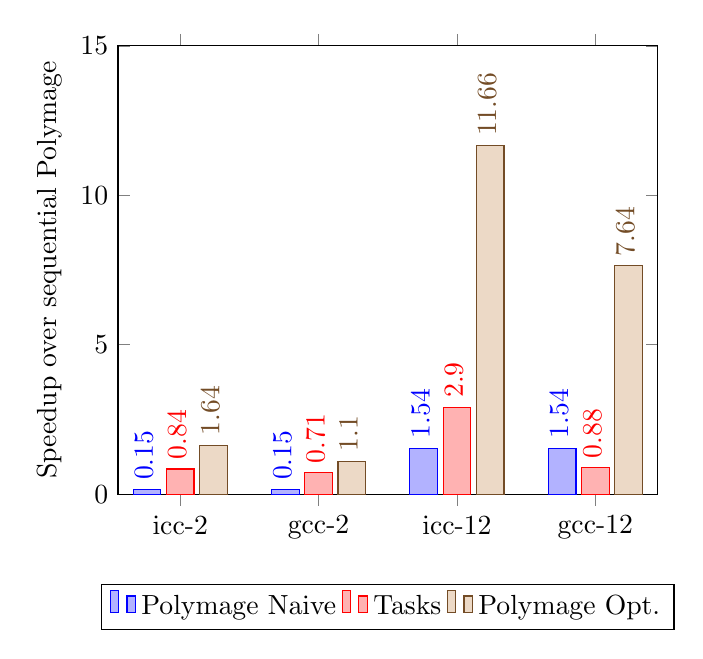
\begin{tikzpicture}
  \centering
  \begin{axis}[
    ybar,
    enlargelimits=0.15,
    enlarge y limits=false,
    ymin=0,
    ymax=15,
     legend style={at={(0.5,-0.2)},
        anchor=north,legend columns=-1},
        ylabel={Speedup over sequential Polymage},
        symbolic x coords={icc-2,gcc-2,icc-12,gcc-12},
      xtick=data,
        nodes near coords,
    every node near coord/.append style={
        anchor=mid west,
        rotate=90
    }
    ]
    \addplot coordinates {(icc-2,0.15)(gcc-2,0.15)(icc-12,1.54)(gcc-12,1.54)};
    \addplot coordinates {(icc-2,0.84)(gcc-2,0.71)(icc-12,2.9)(gcc-12,0.88)};
    \addplot coordinates {(icc-2,1.64)(gcc-2,1.1)(icc-12,11.66)(gcc-12,7.64)};
    \legend{Polymage Naive, Tasks, Polymage Opt.}
  \end{axis}
\end{tikzpicture}
  \end{center}
  \caption{Speedup relative to sequential Polymage, on machines with 2 and 12 cores,
with \texttt{gcc 4.9.1} and \texttt{icc 15.1}.}
  \label{results_hcd}
\end{figure}

The algorithm using tasks does not perform as well as the optimized version from Polymage. 
The gain from the absence of redundant computation, and a potential good reuse
of memory in task scheduling does not compensate the loss due to more synchronization
and fused-loops distribution. But the excellent performance of Polymage, nearly scaling
linearly with the number of cores (see [11] for more results) also relies on good compiler
optimizations of the heavily computational step resulting from loop-fusion.\\
We tried to measure performance without advanced compiler optimizations, using \texttt{-O2} for
\texttt{gcc} and \texttt{icc}. This disables automatic loop vectorization. Since most of the time 
is spent in the computational fused loops, performance is badly reduced and parallel implementations
of Harris Corner Detection are slower than the sequential with automatic vectorization. 
But the version using OpenMP tasks performs better without compiler vectorization than
Polymage version using heavily fused loops. \\
The different implementations are available on Github at :\\
\texttt{https://github.com/victornicolet/harris-corner-implementations},\\
with both the sources from Polymage and the algorithm using tasks.



%********************************************************
%  1-d jacobi
%********************************************************
\section{1-d Jacobi}
Time iterated stencils can be good candidates for an efficient use of tasks. Here we are
interested in small iteration numbers, and we implement a specific tiling strategies in this
case. \\
The OpenMP implementations are available at \\
\texttt{http://www.github.com/victornicolet/tiling-strategies},\\
along with some results.

\subsection{Half-diamonds tiling}
Diamond tiling has proven an efficient tiling strategy since it provides a concurrent start,
locality and possible reuse. In out case, we consider only cases when the number of
iterations is low. The iteration space is tiled using hyperplanes $(1, 1)$ and $(−1, 1)$ as
shown in figure 13. We easily show the legality of this tiling since with the provided
hyperplanes. For each statement S with the tiling hyperplanes for each dependency $d \in
{(−1, 1), (0, 1), (1, 1)}$  we have $h1 \cdot d \geq 0$ and $h2 \cdot d \geq 0$ . \\

\begin{figure}[h]
  \begin{center}
  % \usepackage[usenames,dvipsnames]{pstricks}
% \usepackage{epsfig}
% \usepackage{pst-grad} % For gradients
% \usepackage{pst-plot} % For axes
% User Packages:
% 
% 
\psscalebox{.7 .7} % Change this value to rescale the drawing.
{
\begin{pspicture}(0,-2.52)(16.81,2.52)
\definecolor{colour1}{rgb}{0.7411765,0.7411765,0.7411765}
\definecolor{colour0}{rgb}{0.003921569,0.003921569,0.003921569}
\psline[linecolor=black, linewidth=0.04, arrowsize=0.05291666666666667cm 2.0,arrowlength=1.4,arrowinset=0.0]{->}(2.0,-1.32)(2.0,2.28)
\psline[linecolor=black, linewidth=0.04, arrowsize=0.05291666666666667cm 2.0,arrowlength=1.4,arrowinset=0.0]{->}(2.0,-1.32)(16.8,-1.32)
\pstriangle[linecolor=black, linewidth=0.04, fillstyle=crosshatch, hatchwidth=0.028222222, hatchangle=0.0, hatchsep=0.1411111, hatchcolor=colour1, dimen=outer](5.2,-1.32)(6.4,2.8)
\pstriangle[linecolor=black, linewidth=0.04, fillstyle=crosshatch, hatchwidth=0.028222222, hatchangle=0.0, hatchsep=0.1411111, hatchcolor=colour1, dimen=outer](11.6,-1.32)(6.4,2.8)
\pspolygon[linecolor=black, linewidth=0.04, fillstyle=crosshatch, hatchwidth=0.028222222, hatchangle=0.0, hatchsep=0.1411111, hatchcolor=colour1](14.8,-1.32)(16.4,0.28)(16.4,-1.32)
\psline[linecolor=black, linewidth=0.04](2.0,1.48)(16.0,1.48)
\psline[linecolor=red, linewidth=0.074, arrowsize=0.05291666666666667cm 2.0,arrowlength=1.4,arrowinset=0.0]{->}(4.0,-0.52)(3.2,0.28)
\psline[linecolor=red, linewidth=0.074, arrowsize=0.05291666666666667cm 2.0,arrowlength=1.4,arrowinset=0.0]{->}(6.4,-0.52)(7.2,0.28)
\psline[linecolor=red, linewidth=0.074, arrowsize=0.05291666666666667cm 2.0,arrowlength=1.4,arrowinset=0.0]{->}(10.4,-0.52)(9.6,0.28)
\psline[linecolor=red, linewidth=0.074, arrowsize=0.05291666666666667cm 2.0,arrowlength=1.4,arrowinset=0.0]{->}(12.8,-0.52)(13.6,0.28)
\psline[linecolor=red, linewidth=0.074, arrowsize=0.05291666666666667cm 2.0,arrowlength=1.4,arrowinset=0.0]{->}(16.0,-0.52)(15.2,0.28)
\rput[bl](0.0,2.28){iterations}
\psline[linecolor=red, linewidth=0.074, arrowsize=0.05291666666666667cm 2.0,arrowlength=1.4,arrowinset=0.0]{->}(3.2,-2.12)(4.8,-2.12)
\rput(6.8,-2.12){\textcolor{colour0}{inter-tile dependency}}
\psframe[linecolor=colour0, linewidth=0.042, dimen=outer](8.8,-1.72)(2.8,-2.52)
\rput[bl](16.0,-1.72){\textcolor{colour0}{space}}
\rput[bl](0.4,1.48){\textcolor{colour0}{$i_{max} - 1$}}
\rput[bl](1.2,-1.32){\textcolor{colour0}{0}}
\end{pspicture}
}
  
  \end{center}
  \caption{Half-diamonds tiling for low-iterations stencil computations}
  \label{hdiam_tiling}
\end{figure}


We have implemented a first naive version, using a global barrier between lower and
upper tiles, and static scheduling. Even if this tiling seems quite simple, hand-writing
tiled loops is quite tricky. This version has a few errors on the borders of the array, but
these errors should not affect performance in any way. \\
\paragraph{Grouping tiles} take advantage of the memory architecture and fast L1 caches, it can be
more interesting to adjust the size of the chunks in the loops, and the execution schedule.
In the previous version, if the data size is significantly greater than the lower caches, the
memory of the first lower tiles will be flushed out the caches before being reused by the
upper tiles. To solve this problem, we group loop parts together, adjusting their size proportionally 
to the number of physical cores of the platform. The goal is to take advantage
of static scheduling, which distributes evenly chunks of the loop across processing units to
specify exactly how much computation we want to distribute. The group size is calculated
depending on the number of processors $n_{cores}$ , the size of the L1 cache and the size of the
tile in memory (the size of the array containing the temporary elements between lower
and upper tiles) :
\[Group \ size = n_{cores} ∗ (L1 \ cache \ size) / (tile \ size \  in \  memory)\]

\paragraph{Results} The tiling for low iteration numbers without grouping tiles has proven efficient,
scaling well with the number of processors. But the expected gain with grouping tiles
has not been observed. The version with grouped tiles performs similarly to the simpler
version, with a constant overhead. The schedule on the implementation
with a global barrier between lower and upper tiles is already taking advantage of reuse
through a good mapping of tiles on the threads. \\
We still need to determine why grouping the tile into a size fitting the fastest cache
level does not improve the performance, since it should improve reuse. Varying the group
size does not affect performance either, even if the tile scheduling on the different processor
is as expected : in each group upper tiles are executed on the same core as the lower tiles
at their right.

\subsection{A task-based approach}
We wanted to show that the scheduler can improve data reuse in caches as much as the static 
scheduling with grouping by using a task approach. We build the tasks with
one lower tile and the upper tile immediately to its left. \\
Taking the left tile will reduce task stalling : the data dependency will probably be satisfied 
by the left task before the current task  begins to compute its upper tile. In 
figure~\ref{hdiam_tasking} we summarize the task graph construction: each task 
spawns its successor immediately after starting, then computes the lower tile and 
stalls at the barrier if the left task has not finished to compute the upper
tile. The upper half-tiles at the borders of the domain are treated separately.\\
Data reuse can be exploited at the border between upper and lower tiles, by executing
neighboring tasks on the same processor. But the scheduler has to keep computational
load balanced between the different processors.

\begin{figure}[h]
 % \usepackage[usenames,dvipsnames]{pstricks}
% \usepackage{epsfig}
% \usepackage{pst-grad} % For gradients
% \usepackage{pst-plot} % For axes
% User Packages:
% 
% 
\psscalebox{1.0 1.0} % Change this value to rescale the drawing.
{
\begin{pspicture}(0,-3.5534792)(14.344269,3.5534792)
\definecolor{colour1}{rgb}{0.7490196,0.7490196,0.7490196}
\definecolor{colour0}{rgb}{0.003921569,0.003921569,0.003921569}
\pspolygon[linecolor=black, linewidth=0.04, fillstyle=crosshatch, hatchwidth=0.028222222, hatchangle=0.0, hatchsep=0.1411111, hatchcolor=colour1](6.0373106,-2.3534791)(3.6373105,1.2465209)(8.43731,1.2465209)(10.837311,-2.3534791)(10.037311,-2.3534791)
\psline[linecolor=black, linewidth=0.04, arrowsize=0.05291666666666667cm 2.0,arrowlength=1.4,arrowinset=0.0]{<-}(0.037310485,3.6465209)(0.037310485,-2.3534791)
\psline[linecolor=black, linewidth=0.04, arrowsize=0.05291666666666667cm 2.0,arrowlength=1.4,arrowinset=0.0]{<-}(14.43731,-2.3534791)(0.037310485,-2.3534791)
\psline[linecolor=black, linewidth=0.04, linestyle=dashed, dash=0.17638889cm 0.10583334cm](0.8373105,-2.3534791)(3.6373105,1.2465209)
\psline[linecolor=black, linewidth=0.04, linestyle=dashed, dash=0.17638889cm 0.10583334cm](6.0373106,-2.3534791)(8.43731,1.2465209)
\psline[linecolor=black, linewidth=0.04](3.6373105,1.2465209)(0.037310485,1.2465209)
\psline[linecolor=black, linewidth=0.04](8.43731,1.2465209)(12.837311,1.2465209)
\psline[linecolor=black, linewidth=0.04](0.8373105,-2.3534791)(0.037310485,-1.1534791)(0.037310485,-1.1534791)
\psline[linecolor=black, linewidth=0.04, linestyle=dashed, dash=0.17638889cm 0.10583334cm](10.837311,-2.3534791)(12.037311,-0.7534792)
\psline[linecolor=black, linewidth=0.096, arrowsize=0.05291666666666667cm 2.0,arrowlength=1.4,arrowinset=0.0]{->}(4.4373107,-0.7534792)(5.6373105,0.046520844)
\psline[linecolor=black, linewidth=0.096, arrowsize=0.05291666666666667cm 2.0,arrowlength=1.4,arrowinset=0.0]{->}(9.23731,-0.7534792)(10.43731,0.046520844)
\psbezier[linecolor=red, linewidth=0.08, linestyle=dashed, dash=0.17638889cm 0.10583334cm, arrowsize=0.05291666666666667cm 2.0,arrowlength=1.4,arrowinset=0.0]{->}(1.2373105,-2.3534791)(1.6373105,-3.5534792)(6.0373106,-3.5534792)(6.4373107,-2.3534791)
\psbezier[linecolor=red, linewidth=0.08, linestyle=dashed, dash=0.17638889cm 0.10583334cm, arrowsize=0.05291666666666667cm 2.0,arrowlength=1.4,arrowinset=0.0]{->}(6.8373103,-2.3534791)(7.2373104,-3.153479)(10.837311,-3.5534792)(11.23731,-2.3534791)
\psline[linecolor=colour0, linewidth=0.042, arrowsize=0.05291666666666667cm 2.0,arrowlength=1.4,arrowinset=0.0]{->}(6.4373107,2.046521)(6.4373107,-0.35347915)
\rput[bl](6.0373106,2.4465208){\textcolor{colour0}{barrier}}
\rput[bl](10.43731,-0.7534792){\textcolor{colour0}{data dependency}}
\rput[bl](10.837311,-3.5534792){\textcolor{colour0}{spawning task}}
\end{pspicture}
}

 \caption{Tasks dependencies, synchronization points and creation schema}
 \label{hdiam_tasking}
\end{figure}


\subsection{First results}

This first version uses fixed-shape tiles : half diamonds with fixed hyperplanes, only the
width varies depending on the number of iterations. It does not perform well compared to
the statically scheduled OpenMP reference we use with the same tiling. On small iteration
numbers the task version is slower than the sequential version. It can be explained by the
granularity of the execution : the tasks are very small when the number of iterations is small.
The time spent in the computation is mostly spent in scheduling: the runtime manages many tasks,
which terminate very rapidly. \\
The performance of the scheduler measured with this implementation with such very small
tasks was still better than OpenMP4’s using tasks pragmas.

\subsection{Tile shape determination at runtime}
The previous results showed that the runtime was under performing because of the high
granularity of the task graph. Since our tiling was designed for small iteration numbers,
the tile sizes were relatively small in terms of memory occupation and computational
weight. \\
With tiles of variable size shaped at runtime, depending on the number of iterations, we
can increase the weight of this tasks. Similarly to the computation of group size in the
previous section,the tile size depends on the size of the cache to ensure a good locality, and
that sufficient time is spent in the task. We vary the orientation of the oblique hyperplanes
with a slope between 1 (as in the previous version) and a value so that there is enough tiles
to be distributed among the working threads. Tiling hyperplanes normal vectors are now 
$\vec{h1} = (−a, 1)$ and $\vec{h2} = (a, 1)$ with $1/a = n_{cores} \times (L1 \ cache \ size) / 
(tile \ size \ in  \ memory)$.
This tiling is still legal and valid with $a \leq 1$, the scalar product between dependencies and
hyperplanes normal vectors is positive or null. \\
The only change using this tiling is the amount of computation in each tile. We can
fear that using this skewed tiling space with large strides in the inner-tile time loop 
could lead to worse compiler automatic vectorization. \\
This technique combined with the task approach to this problem has given better results, in
par with OpenMP on small problems but performing better with increasing sizes, showing
speedups better than linearly-increasing with the number of cores. On the 12-core machine
with a problem size of 32 MB, we reached speedups up to 20 times better than sequential,
3 times better than OpenMP. The results are shown in figure~\ref{results_hdiam_var}. \\
To calculate the speedups, the execution times of OpenMP and Libkpn implementations have 
been compared with a sequential  version of 1-d jacobi, without tiling or any optimization.
This can explain the speedups greater than the number of cores. This results still need to be
validated with a more rigorous method.\\
We have bad performance with small iteration sizes and small space sizes. This may be
coming from the lack of parallelism with a number of tasks too small because the slope
of the sides of the tiles was not bounded : for small iterations, the tile is very wide
and it could span a large part of the space. \\
The final program at the moment I am writing this report still contains a few errors, 
concerning the correctness of the output, but they do not affect performance in any way. 
They come from the hand-tuned loops during the tiling and transformations, a process 
that we seek to automate through polyhedral code generation tools and
compilation. The main goals here were to show a well performing tiling for time-iterated
stencils, and validate the approach of implementing the algorithm using lightweight tasks
and dynamic scheduling instead of the classical approach with static scheduling through
loop-chunk distribution.
\begin{figure}[h]
  \begin{center}
  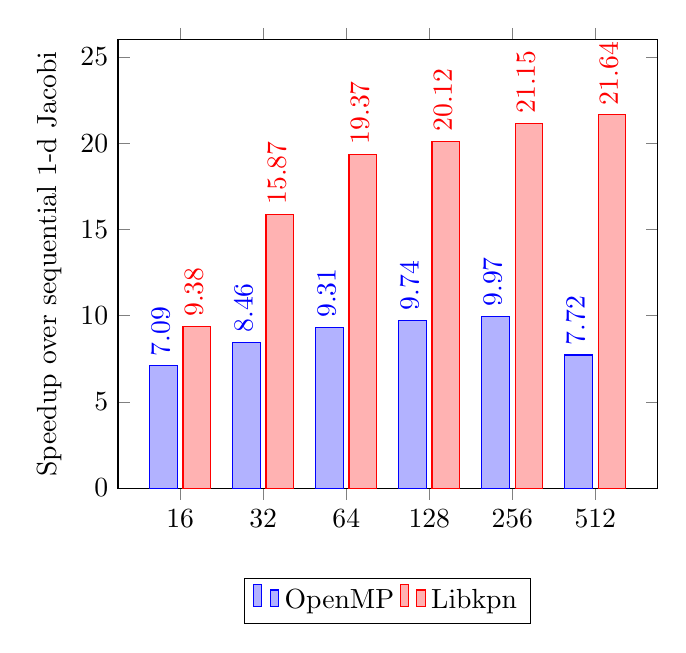
\begin{tikzpicture}
  \centering
  \begin{axis}[
    ybar,
    enlargelimits=0.15,
    enlarge y limits=false,
    ymin=0,
    ymax=26,
     legend style={at={(0.5,-0.2)},
        anchor=north,legend columns=-1},
        ylabel={Speedup over sequential 1-d Jacobi},
        symbolic x coords={16,32,64,128,256,512},
      xtick=data,
        nodes near coords,
    every node near coord/.append style={
        anchor=mid west,
        rotate=90
    }
    ]
    \addplot coordinates {(16,7.09)(32,8.46)(64,9.31)(128,9.74)(256,9.97)(512,7.72)};
    \addplot coordinates {(16,9.38)(32,15.87)(64,19.37)(128,20.12)(256,21.15)(512,21.64)};
    \legend{OpenMP, Libkpn}
  \end{axis}
\end{tikzpicture}
  \end{center}
 \caption{Speedup relative to sequential 1-d jacobi on 12 cores, with different iteration 
 sizes on a 32 Mb problem.}
 \label{results_hdiam_var}
\end{figure}

\newpage
\section{Conclusion and future work}
My internship had a strong experimental component but I also learned a lot on the theoretical point
of view. \\
Optimization is a very experiment field, and I used various tools to validate of refute the 
hypothesis, and to confirm optimization choices. Part of the time I spent on the applications for task
parallelism was dedicated to profiling and debugging to understand what was happening during the concurrent
computations.\\
The bibliographic study of concurrent parallelism lead me to a better understanding of the different
models I was working with (OpenMP and Libkpn). This was necessary for both developing the applications
and analyzing their performance, as well as very enriching given my interest in computer science.\\
The first results with Harris Corner Detection were not satisfying but provided me the tools
for the next application. The results presented are yet to be confirmed with a more rigorous 
experiment, but they are the outcome of a sequence of benchmarking and analysis.\\
A the time of writing this report, my internship is not finished yet. There is still work to be done
concerning the validation of the last results, and on their analysis, especially concerning the relation 
between the slope in the tile shape and performance with automatic vectorization. I consider this
as a good experience of experimental research work.\\
Finally, this internship might be part of future work. Testing Libkpn on 1-d jacobi was only an example,
since this application is too simple and not very used in real scientific computations. More pertinent
applications need to be implemented in order to lead to a publication.


\newpage
\section{References}
\bibliography{internship_report.bib}
\end{document}
